\chapter{Top Asymmetry Measurements}
\label{chap:afb}

This chapter will describe the measurements of several asymmetries in
events where a top-antitop ($\ttbar$) pair decays to a two-lepton
final state ($2\ell$). This work was performed during Run I of the LHC and the
CMS detector, at both 7 TeV and 8 TeV center-of-mass energies, though
I will focus on the 8 TeV results, and in particular, my work on the
unfolding technique. The 8 TeV analysis led to two publications, which
are Refs. \cite{chargeasym} and \cite{spincorrpol}.

% Question: Should I use the past tense of present tense when
% describing this analysis?
% I guess the same question is also applicable to the stop analysis.

\section{Motivation}
\label{sec:afbmotivation}

As mentioned in Section \ref{ssec:SMdescription}, the top quark is the
heaviest known elementary particle, with a mass of $\sim 173$ GeV
\cite{pdg}. This large mass gives the top quark a number of properties
that make it uniquely interesting to study.

In particle physics, a particle's mass is inversely proportional to
its lifetime - how long it tends to last before decaying. % Do I need a citation for this?
Because the top quark is so heavy, it has an extremely short lifetime
of $\mathcal{O} (10^{-25})$ seconds \cite{pdg}.
Because this lifetime is so short, there is insufficient time for the
top quark to hadronize, or for spin decorrelation to occur. % Does this need a separate reference?
Thus, unlike any other quark, the polarization and spin correlation
of the top quark are preserved in its decay products. So by studying
the decays of top quarks, we can learn about the properties of the
bare quark itself.

Additionally, the top quark's large mass places it on the edge of
unexplored territory.
Because the likelihood of a particular decay is proportional
to the mass difference between the particles involved, there are many
models of new physics that predict new particles with a strong
coupling to the top quark. % Probably gonna need to cite or rewrite that claim...
These couplings would naturally cause some of the top quark's
properties to deviate from the value predicted by the SM. Thus, it is
important to make precise measurements of properties such as charge
asymmetry to tease out any links to possible new physics.

% Should talk about why we use the dilepton final state
% And also include a Feynman diagram of the process

\section{Previous Measurements}
\label{sec:afbtevatron}

The Tevatron collider at Fermilab has made several previous measurements of
top charge asymmetry (CITATIONS), and of top spin % Pull in all these citations
correlation and polarization (CITATIONS). The
early charge asymmetry measurements were particularly interesting, because
they revealed a $2\sigma$ deviation from the SM expectation (though
later results, such as Reference (CITATION), showed a
reduced discrepancy). During the LHC Run I, it was
natural to want to confirm the Tevatron measurements, and to extend
them if possible.

The Tevatron collided beams of protons against beams of
antiprotons. When such $p\bar{p}$ collisions produce
$\ttbar$ pairs, we naturally expect the top will travel more along the direction
of the proton beam, and the antitop will travel
more along the direction of the antiproton beam, so that the
difference in their rapidities is positive ($y_t - y_{\bar{t}} > 0$).
This case was called ``forward'', and the reverse was called
``backward''. Thus, given a number of $\ttbar$
events from the Tevatron, we can define a forward-backward
asymmetry by subtracting the number of backward events from the number
of forward ones:

\begin{equation}
A_{FB} = \asymmetry{\Delta y}{0}
\end{equation}

However, the LHC is a proton-proton collider, and as such, there is no
naturally favored direction for the top or antitop to travel. As the
next section will explain, we must define ``forward'' and ``backward''
events somewhat differently.

\section{Asymmetry Variables}
\label{sec:afbvariables}

In this analysis, we evaluated six different asymmetries in $\ttdilep$
events, including two charge asymmetries, one
polarization, and three measures of spin correlation. If any of these
variables deviate from their expected SM values, it could potentially
be a sign of new physics.

\subsection{Definitions}
\label{ssec:afbvariables}

% Top charge asymmetry %%%%%%%%%%%
As at the Tevatron, the top charge asymmetry was measured at CMS using
the rapidity of the top quarks. However, absent a natural direction
for the top and antitop to travel, we categorized events as
``forward'' and ``backward'' based on which quark had a higher
absolute value of rapidity. Thus we define our \textbf{top charge
asymmetry} as:
\begin{equation}
A_C = \asymmetry{|y_t|}{|y_{\bar{t}}|}
\end{equation}

% Leptonic charge asymmetry %%%%%%%%
In addition to the top charge asymmetry, we define a similar
\textbf{leptonic charge asymmetry} to be:
\begin{equation}
A_C^{lep} = \asymmetry{|\eta_{\ell^+}|}{|\eta_{\ell^-}|}
\end{equation}
Though similar to the top charge asymmetry, this variable
is based purely on the pseudorapidity of the leptons produced in the
decay. We may use the leptons as a proxy for the tops because we
expect their direction to be correlated with the directions of their
parent tops. One advantage of using only the leptons is that it obviates the
need to reconstruct the $\ttbar$ system, as described in Sec.
\ref{sec:afbselections}, thereby allowing us to include more events in
our calculation of this variable. However, this variable also has some
dependence on the polarization, so it is not fully correlated with $A_C$.

% INTERLUDE: Helicity angle %%%%%%%%%%%
Before proceding further, we must define the \emph{helicity angle}, which
will be used in the next two asymmetry variables.
The helicity angle $\theta^*_{\ell}$ is defined as the angle
a charged lepton makes in the rest frame of its parent top,
relative to the parent top's direction in the $\ttbar$ center-of-mass
(CM) reference frame. This angle may be defined separately for the
positive and negative charged lepton in an event.

% Top polarization %%%%%%%%%%%%%%
The \textbf{top polarization} is an asymmetry based on the helicity %% Note: revisit this later, and decide whether to present +/- separately or together
angles of the charged leptons, and is given by:
\begin{equation}
A_{P\pm} = \asymmetry{\cos(\theta^*_{\ell^\pm})}{0}
\end{equation}
We measure it for the positively and
negatively charged leptons separately. A different, commonly used
polarization variable, $P$, can be calculated as $P = 2 A_P = 2(
A_{P+} + A_{P-})$, if we assume CP-invariance.

% Top spin correlation %%%%%%%%%
Our \textbf{top spin correlation} asymmetry, which also depends on the
lepton helicity angles, is defined as:
\begin{equation}
A_{c1c2} = \asymmetry{\cos(\theta^*_{\ell^+}) \times \cos(\theta^*_{\ell^-})}{0}
\end{equation}
From this variable, we may also obtain the $C$ spin correlation
coefficient, which is given by $C = -4 \times A_{c1c2}$ \cite{spincorrpolcoeff}.

% Lepton azimuthal asymmetry %%%%%
We also obtain an indirect measurement of the spin correlation using
the \textbf{lepton azimuthal asymmetry}. This variable depends on the
azimuthal angle between the two leptons, and is defined as:
\begin{equation}
A_{\Delta\phi} = \asymmetry{\Delta\phi_{\ell^+\ell^-}}{\pi/2}
\end{equation}
As with the leptonic charge asymmetry, this variable also relies
solely on the charged leptons, and does not require reconstruction of
the $\ttbar$ system, permitting us to use more events than are
available for the top spin correlation.

% Lepton opening angle %%%%%%%%%
Finally, we define our \textbf{lepton opening angle} asymmetry as:
\begin{equation}
A_{\cos\phi} = \asymmetry{\cos(\theta_{\ell\ell})}{0}
\end{equation}
This variable is based on the opening angle between the two leptons in
their respective parent top reference frames. From this measured
asymmetry, we can calculate the $D$ spin correlation coefficient to be
$D = -2 \times A_{\cos\phi}$ \cite{spincorrpolcoeff}.

\subsection{Differential Measurements}
\label{ssec:afbvarsdifferential}

In addition to measuring the above six asymmetries in one dimension
(\emph{inclusively}), we also measured them in two dimensions
(\emph{differentially}), against other physical variables.
We chose to make differential measurements because the CDF charge asymmetry
discrepancy was more pronounced at $\ttbar$ invariant masses above 450 % Cite CDF charge asymmetry at Mtt>450
GeV than below it. If similar behavior occurs at CMS, in any variable,
we would like to observe it. We measured all six of our asymmetry
variables differentially with respect to the $\ttbar$ invariant mass
($m_{\ttbar}$), rapidity ($y_{\ttbar}$), and transverse momentum ($p_T^{\ttbar}$).

\section{Datasets and Triggers}
\label{sec:afbdatatrig}

For this analysis, we used 19.5 fb\textsuperscript{-1} of data from
the 8 TeV portion of CMS Run I, encompassing the 2012A through 2012D
eras. Because the analysis focused on a process that produced two
leptons in the final state, we used the dilepton datasets from that
period. A complete list is given in Table \ref{tab:afb:datasamples}.

%% Table of data samples. Taken from AN-14-246. Believed unpublished so far %%%%%%%
\begin{table}[!ht]
\begin{center}
\caption{List of CMS datasets used.}
\label{tab:afb:datasamples}
{\footnotesize
\begin{tabular}{l|r}
\hline
Dataset Name & run range \\
\hline\hline
Dilepton Samples \\
\hline

  /DoubleMu/Run2012A-13Jul2012-v1/AOD &  190456-193621 \\
  /DoubleElectron/Run2012A-13Jul2012-v1/AOD & 190456-193621  \\
  /MuEG/Run2012A-13Jul2012-v1/AOD & 190456-193621 \\

  /DoubleMu/Run2012A-recover-06Aug2012-v1/AOD & 190949 190945 190906 190895 190782 \\
  /DoubleElectron/Run2012A-recover-06Aug2012-v1/AOD & 190949 190945 190906 190895 190782 \\
  /MuEG/Run2012A-recover-06Aug2012-v1/AOD & 190949 190945 190906 190895 190782\\

  /DoubleElectron/Run2012B-13Jul2012-v1/AOD  & 193834-196531 \\
  /DoubleMu/Run2012B-13Jul2012-v1/AOD  & 193834-196531  \\
  /MuEG/Run2012B-13Jul2012-v1/AOD  & 193834-196531  \\

  /DoubleElectron/Run2012C-24Aug2012-v1/AOD &  197770- 198913 \\
  /DoubleMu/Run2012C-24Aug2012-v1/AOD &  197770- 198913 \\
  /MuEG/Run2012C-24Aug2012-v1/AOD &  197770- 198913 \\

  /DoubleElectron/Run2012C-PromptReco-v2/AOD & 198934 - 203755  \\
  /DoubleMu/Run2012C-PromptReco-v2/AOD &  198934 - 203755 \\
  /MuEG/Run2012C-PromptReco-v2/AOD &  198934 - 203755 \\

  /DoubleElectron/Run2012D-PromptReco-v1/AOD & 203768 - 208686 \\
  /DoubleMu/Run2012D-PromptReco-v1/AOD & 203768 - 208686 \\
  /MuEG/Run2012D-PromptReco-v1/AOD & 203768 - 208686 \\

\hline
\end{tabular}
}
\end{center}
\end{table}

We used several Monte Carlo datasets to model both the $\ttdilep$
process and any potential background processes. A list of all Monte
Carlo datasets used is given in Table \ref{tab:afb:mcsamples}.

%% Table of MC samples. Adapted from AN-14-246. Believed unpublished so far %%%%%%%
\begin{table}[!ht]
\begin{center}
\caption{List of CMS Monte Carlo samples used.}
\label{tab:afb:mcsamples}
{\footnotesize
\begin{tabular}{l|l|c}
\hline
\multicolumn{3}{c}{With Pileup: Processed dataset name is} \\
\multicolumn{3}{c}{(53) Summer12\_DR53X-PU\_S10\_START53\_V7A-v*/AODSIM} \\
\hline
 Description                     &   Primary Dataset Name   & cross-section [pb]\\
\hline
$\ttbar$                                                     &   /TT\_TuneZ2Star\_8TeV-mcatnlo (S3)                            & 234 \\
$\ttbar$ (alternative)                                           &   /TT\_CT10\_TuneZ2Star\_8TeV-powheg-tauola (53)           & 234 \\
W $\rightarrow$ $\ell\nu$+ jets                &   /WJetsToLNu\_TuneZ2Star\_8TeV-madgraph-tarball                             & 37509\\
W $\rightarrow$ $\ell\nu$+1 jets               &   /W1JetsToLNu\_TuneZ2Star\_8TeV-madgraph-tauola (53)                        &  6663  \\
W $\rightarrow$ $\ell\nu$+2 jets               &   /W2JetsToLNu\_TuneZ2Star\_8TeV-madgraph-tauola (53)                        &  2159 \\
W $\rightarrow$ $\ell\nu$+3 jets               &   /W3JetsToLNu\_TuneZ2Star\_8TeV-madgraph-tauola (53)                        &   640 \\
W $\rightarrow$ $\ell\nu$+$\geq 4$ jets        &   /W4JetsToLNu\_TuneZ2Star\_8TeV-madgraph-tauola (53)                        &   264 \\
WW      & /WWJetsTo2L2Nu\_TuneZ2star\_8TeV-madgraph-tauola (53) &   5.8123\\
WZ      & /WZJetsTo3LNu\_TuneZ2\_8TeV-madgraph-tauola (53)              &   1.0575\\
        & /WZJetsTo2L2Q\_TuneZ2star\_8TeV-madgraph-tauola (53)          &   2.206\\
ZZ      & /ZZJetsTo2L2Nu\_TuneZ2star\_8TeV-madgraph-tauola (53)         &   0.365\\
        & /ZZJetsTo4L\_TuneZ2star\_8TeV-madgraph-tauola (53)            &   0.176908\\
        & /ZZJetsTo2L2Q\_TuneZ2star\_8TeV-madgraph-tauola (53)          &   2.4487\\
$WG^{*}$  & /WGstarToLNu2E\_TuneZ2star\_8TeV-madgraph-tauola (53)          &  \\
        & /WGstarToLNu2Mu\_TuneZ2star\_8TeV-madgraph-tauola (53)          &  \\
        & /WGstarToLNu2Tau\_TuneZ2star\_8TeV-madgraph-tauola (53)          &  \\
$t$ ($s$-chan)                           &   /T\_TuneZ2Star\_s-channel\_8TeV-powheg-tauola (53)                        &  3.9 \\
$\bar{t}$ ($s$-chan)                     &   /Tbar\_TuneZ2Star\_s-channel\_8TeV-powheg-tauola (53)                      &  1.8 \\
$t$ ($t$-chan)                           &   /T\_TuneZ2Star\_t-channel\_8TeV-powheg-tauola (53)                         &  55.5 \\
$\bar{t}$ ($t$-chan)                     &   /Tbar\_TuneZ2Star\_t-channel\_8TeV-powheg-tauola (53)                      &  30.0 \\
$tW$                                     &   /T\_TuneZ2Star\_tW-channel-DR\_8TeV-powheg-tauola (53)                     &  11.2 \\
$\bar{t} W$                               &   /Tbar\_TuneZ2Star\_tW-channel-DR\_8TeV-powheg-tauola (53)                  &  11.2 \\
Z/$\gamma^* \rightarrow \ell \ell$      & /DYJetsToLL\_TuneZ2Star\_M-10To50filter\_8TeV-madgraph (53)                   &  860.5 \\
Z/$\gamma^* \rightarrow \ell \ell$      & /DYJetsToLL\_TuneZ2Star\_M-50\_8TeV-madgraph-tarball (53)                   &  3532.8 \\
Z/$\gamma^* \rightarrow \ell \ell$+$\geq 1$ jets       & /DY1JetsToLL\_M-50\_TuneZ2Star\_8TeV-madgraph (53)                   &  671.83 \\
Z/$\gamma^* \rightarrow \ell \ell$+$\geq 2$ jets       & /DY2JetsToLL\_M-50\_TuneZ2Star\_8TeV-madgraph (53)                   &  216.76 \\
Z/$\gamma^* \rightarrow \ell \ell$+$\geq 3$ jets       & /DY3JetsToLL\_M-50\_TuneZ2Star\_8TeV-madgraph (53)                   &  61.2 \\
Z/$\gamma^* \rightarrow \ell \ell$+$\geq 4$ jets       & /DY4JetsToLL\_M-50\_TuneZ2Star\_8TeV-madgraph (53)                   &  27.6 \\
$\ttbar W$                                       &   /TTW\_TuneZ2Star\_8TeV-madgraph (53)                   &  0.23 \\
$\ttbar Z$                                       &   /TTZ\_TuneZ2Star\_8TeV-madgraph (53)                   &  0.21 \\
$\ttbar \gamma$                      &   /TTGJets\_TuneZ2Star\_8TeV-madgraph (53)            &  2.166 \\
$\ttbar W W$                                     &   /TTWW\_TuneZ2Star\_8TeV-madgraph (53)        &  0.002037  \\
WWW     & /WWW\_TuneZ2Star\_8TeV-madgraph (53)                  & 0.08058 \\
WWZ     & /WWZNoGstar\_TuneZ2Star\_8TeV-madgraph (53)           & 0.05798 \\
WZZ     & /WZZNoGstar\_TuneZ2Star\_8TeV-madgraph (53)           & 0.01698 \\
ZZZ     & /ZZZNoGstar\_TuneZ2Star\_8TeV-madgraph (53)           & 0.0055269 \\
WWG     & / WWGJets\_TuneZ2Star\_8TeV-madgraph (53)             & 0.528 \\
\hline\hline
\end{tabular}
}
\end{center}
\end{table}

To select events from the datasets listed in
\ref{tab:afb:datasamples}, we used a set of dilepton triggers that
would capture the four possible dilepton flavors. These triggers are
listed in table \ref{tab:afb:triggers}.
% AN also uses this spot to reference where trigger efficiency weights
% are applied later. Should I?

%% Table of triggers used. Taken from AN-14-246. Believed unpublished so far %%%%%%%
\begin{table}[!ht]
\begin{center}
\caption{List of triggers used.}
\label{tab:afb:triggers}
\begin{tabular}{l}
\hline\hline
Triggers   \\
\hline\hline
Dilepton Sample \\
\hline
\footnotesize{\verb=HLT_Mu17_Mu8_v*=}\\
\footnotesize{\verb=HLT_Mu17_Ele8_CaloIdT_CaloIsoVL_TrkIdVL_TrkIsoVL_v*=}\\
\footnotesize{\verb=HLT_Mu8_Ele17_CaloIdT_CaloIsoVL_TrkIdVL_TrkIsoVL*=}\\
\footnotesize{\verb=HLT_Ele17_CaloIdT_CaloIsoVL_TrkIdVL_TrkIsoVL_Ele8_CaloIdT_CaloIsoVL_TrkIdVL_TrkIsoVL_v*=}\\
\hline
\end{tabular}
\end{center}
\end{table}

\section{Object and Event Selection}
\label{sec:afbselections}

We employed a set of physics object and event selections designed to
accept as many $\ttdilep$ events as possible while minimizing the
number of background events selected.

\subsection{Object Definitions}
\label{ssec:afb:objdefs}

For the purpose of our analysis, we consider a lepton to mean an
electron or muon. We define those particles using the following
criteria:

\begin{itemize}
\item Electrons and muons are defined using the recommended
  2012 identification criteria provided by their respective Physics Object
  Groups (POGs) within CMS. Specifically, electrons use the
  recommended medium working point (WP), and muons use the recommended
  tight WP.
\item We require $p_T > 20$ GeV and $|\eta| < 2.4$.
\item We use particle flow-based isolation within a cone of $\Delta R
  < 0.3$, where relative isolation must be $< 0.15$ and absolute
  isolation must be $< 5$ GeV. % AN talks about PU corrections using \Delta\beta
\item The PF lepton and the reconstructed lepton must have $p_T$ that
  differ by $< 10$ GeV.
\item For electrons, we require $E / p_{in} < 4$.
\end{itemize}

Jets are defined using particle flow. They must have $p_T > 30$ GeV
and $|\eta| < 2.4$. They must pass the tight Multi-Variate Analysis
(MVA) pileup ID, and they must be separated from leptons by $\Delta R
> 0.4$. B-tagging of jets is done using the Combined Secondary Vertex
(CSV) medium working point.

MET is computed by summing up the vector momenta of all PF particles,
and multiplying by $-1$.

\subsection{Event Selections}
\label{ssec:afb:eventsel}

Using the above object definitions, we select events with exactly
two leptons of opposite-sign charge, and at least two jets, including at
least one b-tagged jet. Some additional requirements on these objects
include:

\begin{itemize}
\item To discount events with low-mass resonances, we require the
  dilepton invariant mass $M_{\ell\ell} > 20$ GeV.
\item For events where the leptons have the same flavor, we require
  $|M_{\ell\ell} - M_Z| > 15$ GeV to exclude dileptons produced by the
  Drell-Yan (DY) process.
\item We also require MET $> 40$ GeV in same-flavor events, which
  further helps to reduce the DY background.
\end{itemize}

Additionally, we clean our data events using a number of standard
event filters. These filters are:

\begin{itemize}
\item At least one primary vertex
\item Beam scraping events
\item Tracking failure
\item HBHE noise filter
\item EE noise filter
\item ECAL/HCAL laser events
\item CSCHaloFilter
\item Anomalous $\rho$
\end{itemize}

\subsection{Corrections}
\label{ssec:afb:evtweights}

We make several corrections to our data to remove spurious effects,
and to our Monte Carlo simulations to more accurately reflect the
properties of the data. In particular:

\begin{itemize}
\item We evaluate the efficiencies of our chosen triggers,
  parameterized in $p_T$ and $\eta$, and correct
  MC events to reflect these weights. % Do I need to describe this process in detail?
\item We use lepton identification and isolation efficiencies measured
  in a different analysis (CITATION). As these values agree well with % Need citation
  the efficiencies of our MC, we apply no correction, but we do assign
  a systematic uncertainty, as described in Section
  \ref{sec:afbsystematics}.
\item We correct the MC for the efficiency of b-tagging using the CSV
  discriminator reshaping method
\item We apply the standard Jet Energy Corrections (JECs)
\item JECs are propagated to the MET calculation for jets with $p_T >
  10$ GeV, and the MET is also corrected to remove modulation in $\phi$.
\end{itemize}

\subsection{\texorpdfstring{$\ttbar$}{ttbar} System Reconstruction}
\label{ssec:afb:ttbarreconstruction}

For some of the asymmetry variables described in Section
\ref{ssec:afbvariables}, it is necessary to reconstruct the $\ttbar$
system and its decay. This process is challenging because we do not
know the exact momenta of the two neutrinos (only the total MET for
the event), and because there is an ambiguity as to which lepton
corresponds with which b-jet. In addition, some events have only one
medium CSV jet, not two.

In cases with only one medium CSV jet, we treat the next-highest-CSV
jet like a second b-tag. We then plug the two b-jets, the lepton
four-momenta, and the MET into an analytical neutrino solver that
attempts to reconstruct the $\ttbar$ system, assuming a fixed top mass
of 172.5 GeV \cite{nusolver}. Of the up to eight possible solutions
for each event, this software chooses the one with the greatest matrix
weight. In cases where no solution is found, it returns the closest
approach to a real solution. If no closest approach solution is
possible, we do not use the event in measuring the asymmetries that
require $\ttbar$ reconstruction (about 16\% of events, in both data
and MC).

% Do I need to present the efficiency and resolution of the neutrino
% solver? Maybe kick this to an appendix?

\section{Background Estimation}
\label{sec:afbbackground}

In general, the backgrounds in this analysis are estimated using Monte
Carlo simulations, normalized based on next-to leading order (NLO) or
next-to next-to leading order (NNLO) cross sections. However, we
validate these estimates and
derive scale factors (SFs) and uncertainties for the backgrounds by
comparing them to data in certain control regions. Our largest
background is irreducible, namely single-top production
in the $tW$ channel. However, it is documented that this background is
well-modeled by MC, and therefore requires no correction (CITATION). % Citation for TOP-12-040
And fortunately, our measurements depend on the shape of the data, and
thus are not very sensitive to the normalization of the background
components. Finally, as we will see in Section
\ref{sec:afbdatamccompare}, our background yields are very small
compared to the $\ttdilep$ signal.

Since our signal region (SR) is designed to enhance the $\ttdilep$
process and exclude backgrounds, we can create control regions (CRs)
that target specific background processes by inverting one to two cuts
and selections from the SR. There are three broad categories of CRs,
each targeting a particular background component,
outlined in Figure \ref{fig:afb:crs}. These CRs are described in
detail in Table \ref{tab:afb:crdefs}.

% Pulled from AN-14-246. UNPUBLISHED! %%%%%%%%%%%%%%%%%
\vspace{0.25in}
\begin{figure}[t]
  \centering
  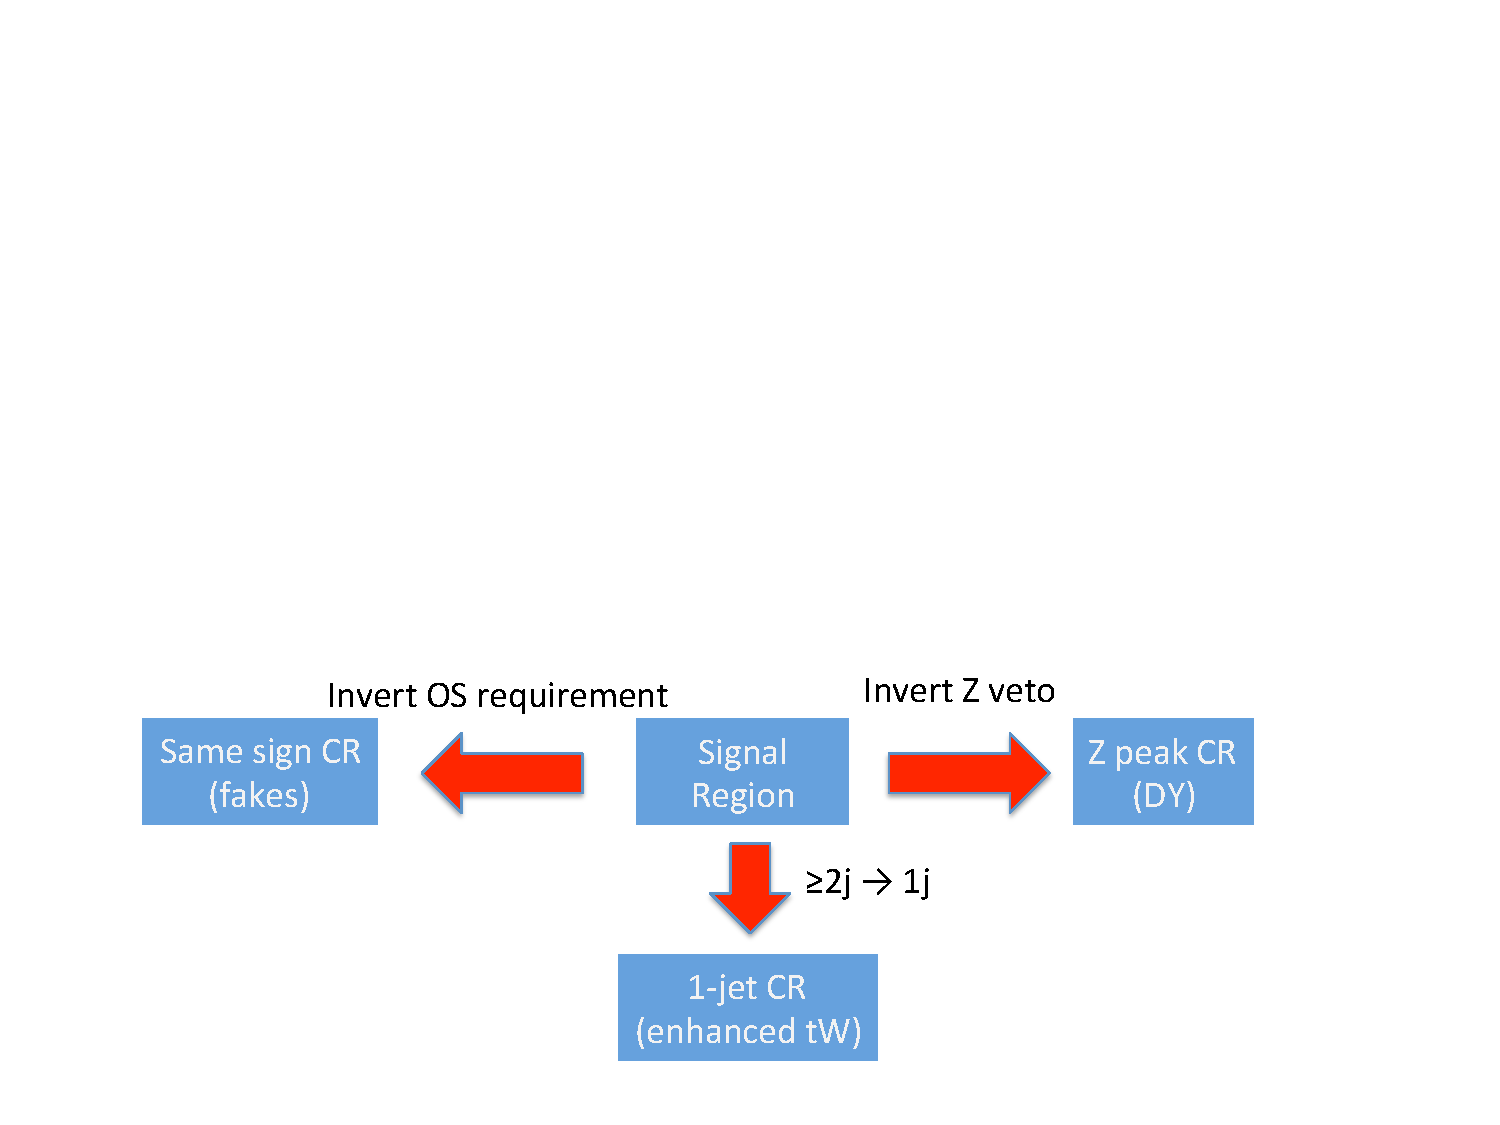
\includegraphics[width=0.75\textwidth]{figures/CRsdef.pdf}
  \caption{Relationships between the SR and the different categories of CRs.}
  \label{fig:afb:crs}
\end{figure}


% Adapted from AN-14-246 UNPUBLISHED! %%%%%%%%%%%%%%%%%%
\begin{table}[h]
\begin{center}
\caption{Summary of control regions. For each ``CR$N$'' other than
  CR0, there is a corresponding ``CR$N$v'', with a b-veto added.}
\label{tab:afb:crdefs}
{\small
\begin{tabular}{l|c c}
\hline
Selection Criteria & Name & Target process  \\
\hline
b veto & CR0 & DY \\
\hline
Z peak & CR1 & DY \\
\hline
Z peak, no MET cut & CR2 & DY \\
\hline
No MET cut & CR3 & DY \\
\hline
1 jet & CR4 & tW  \\
\hline
Same sign & CR5 & Fakes \\
\hline
Same sign, no MET cut & CR6 & Fakes \\
\hline
\end{tabular}
}
\end{center}
\end{table}

In each control region, we vary the normalization of the targeted
background process until the MC yield matches the data yield in that
region. The SF for the DY process is taken from CR1, and the SF for
fakes is taken from CR5; in each case, the related CRs are used to
derive an envelope of variation that defines the systematic
uncertainties on the SFs. These envelopes are depicted in Figure
\ref{fig:afb:sfvariations}, and the final SFs and uncertainties are
given in Table \ref{tab:afb:sfs}. Since we do not apply a SF to the
$tW$ background, we take the uncertainty on this background component
from the uncertainty on a CMS cross section measurement of $23.4 \pm
5.4$ pb \cite{twxsec}.

% Pulled from AN-14-246. UNPUBLISHED! %%%%%%%%%%%%%%%%%
\begin{figure}[t]
  \centering
  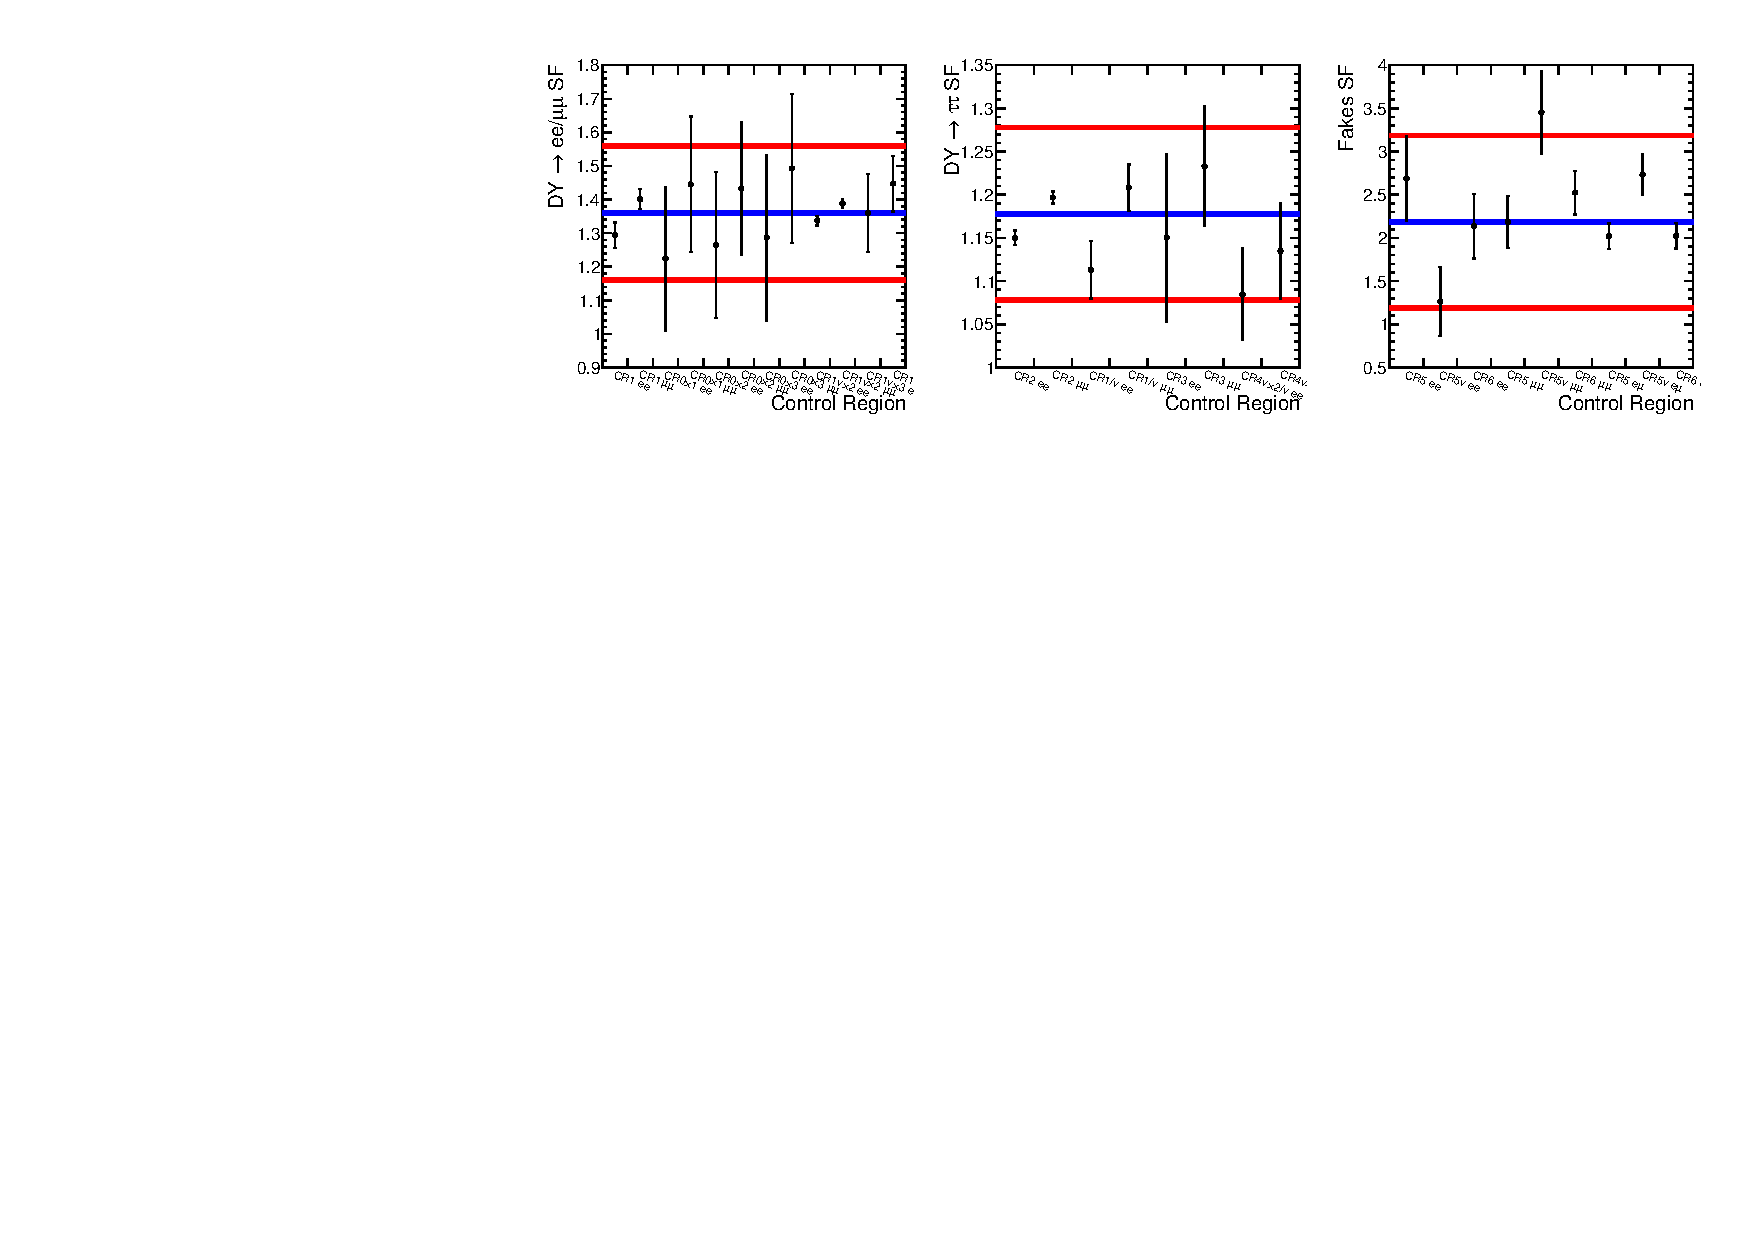
\includegraphics[width=0.75\textwidth]{figures/SFs_all.pdf}
  \caption{SFs measured in different CRs. Blue line depicts the
    central value, and red lines give the systematic uncertainty band.}
  \label{fig:afb:sfvariations}
\end{figure}

% Pulled from AN-14-246. Something similar has been published.
\begin{table}[h]
\begin{center}
\caption{SFs applied to the background components, and their
  associated uncertainties.}
\label{tab:afb:sfs}
{\small
\begin{tabular}{l|c}
\hline
Process & SF  \\
\hline
DY$\rightarrow ee/\mu\mu$ & 1.36 $\pm$ 0.02 (stat) $\pm$ 0.2 (syst) \\
DY$\rightarrow\tau\tau$   & 1.18 $\pm$ 0.01 (stat) $\pm$ 0.1 (syst) \\
fakes             & 2.18 $\pm$ 0.30 (stat) $\pm$ 1.0 (syst) \\
tW                & 1.00 $\pm$ 0.25 (syst) \\
\hline
\end{tabular}
}
\end{center}
\end{table}

\section{Comparison Between Data and Simulation}
\label{sec:afbdatamccompare}

After applying the event selections and scale factors described in the
previous section, our MC-predicted and observed event yields are as
shown in Table \ref{tab:afb:datamcyields}. The dileptonic $\ttbar$
MC has been rescaled so that the total MC yield equals the total data
yield, because we assume that anything that isn't background must be
signal. This $\ttdilep$ sample was generated using MC@NLO, and
required a scale factor of 0.95 to match the data yield. The original
cross section was verified using Powheg. When all is said and done, the
total yield is approximately 91\% signal and 9\% background.

Figure \ref{fig:afb:datamccompare} provides comparisons between data
and Monte Carlo predictions for several of the kinematic variables
that describe the $\ttbar$ system, after all corrections and scale
factors have been applied. As the plots themselves and the associated
ratios show, the MC predictions match the data fairly well, indicating
good quality modeling of the background processes and the
$\ttdilep$ process.

% Adapted from AN-14-246. Similar table published in spin correlation/polarization paper.
\begin{table}[htb]
\begin{center}
\caption{Observed and expected yields after applying preselection and scale
  factors. Yields are scaled to a luminosity of 19.5
  fb\textsuperscript{-1}. Uncertainties are statistical only.}
\label{tab:afb:datamcyields}
\begin{tabular}{l |  c  c  c  c}
\hline
                                        Sample   &                $ee$   &            $\mu\mu$   &              $e\mu$   &               Total  \\
\hline
                 $\ttbar \rightarrow \ell\ell$   &   6313.6 $\pm$ 37.7   &   8975.7 $\pm$ 44.1   &  24651.6 $\pm$ 73.4   &  39940.9 $\pm$ 93.6  \\
              $\ttbar \rightarrow \ell +$ jets   &     107.1 $\pm$ 7.7   &      62.2 $\pm$ 5.4   &    327.4 $\pm$ 13.4   &    496.7 $\pm$ 16.4  \\
                                        W+jets   &       7.3 $\pm$ 3.6   &       1.8 $\pm$ 1.8   &      10.0 $\pm$ 3.5   &      19.1 $\pm$ 5.3  \\
                  single top (s/t-chan, 1-lep)   &       2.6 $\pm$ 0.6   &       4.6 $\pm$ 0.9   &      18.8 $\pm$ 1.6   &      26.1 $\pm$ 1.9  \\
                        single top (tW, 2-lep)   &     298.0 $\pm$ 1.6   &     425.9 $\pm$ 1.9   &    1161.9 $\pm$ 3.1   &    1885.8 $\pm$ 4.0  \\
                                      WW/WZ/ZZ   &      27.6 $\pm$ 1.4   &      40.7 $\pm$ 1.4   &      89.3 $\pm$ 2.3   &     157.5 $\pm$ 3.0  \\
               DY $\rightarrow ee/\mu\mu$+jets   &    211.0 $\pm$ 16.0   &    368.0 $\pm$ 22.8   &       1.6 $\pm$ 0.5   &    580.6 $\pm$ 27.9  \\
                DY $\rightarrow \tau\tau$+jets   &      33.9 $\pm$ 2.5   &      51.5 $\pm$ 3.0   &     137.6 $\pm$ 5.1   &     223.0 $\pm$ 6.4  \\
                                ttW/Z/$\gamma$   &      86.4 $\pm$ 6.5   &     141.3 $\pm$ 8.2   &    331.6 $\pm$ 12.8   &    559.2 $\pm$ 16.5  \\
                                      triboson   &       1.5 $\pm$ 0.1   &       2.3 $\pm$ 0.2   &       5.2 $\pm$ 0.3   &       9.0 $\pm$ 0.4  \\
\hline
                                   Total SM MC   &   7089.0 $\pm$ 42.5   &  10074.0 $\pm$ 50.8   &  26735.0 $\pm$ 76.1   & 43898.0 $\pm$ 100.9  \\
\hline
                                          Data   &                7089   &               10074   &               26735   &               43898  \\
\hline

\end{tabular}
\end{center}
\end{table}

% Pulled from AN-14-246. These exact plots are unpublished, but some similar ones may be published in the spin corr/pol paper. %%%%%%%%%%%%%%%%%
% I'll probably need to change these around to meet criteria for published plots.
\begin{figure}[phtb]
  \centering
  \includegraphics[width=0.45\textwidth]{figures/dataMC/n_bjets_combined.pdf}
  \includegraphics[width=0.45\textwidth]{figures/dataMC/lepPt_combined.pdf}
  \includegraphics[width=0.45\textwidth]{figures/dataMC/met_combined.pdf}
  \includegraphics[width=0.45\textwidth]{figures/dataMC/tt_mass_combined.pdf}
  \includegraphics[width=0.45\textwidth]{figures/dataMC/tt_pT_combined.pdf}
  \includegraphics[width=0.45\textwidth]{figures/dataMC/ttRapidity2_combined.pdf}
  \caption{Comparison of data with Monte Carlo predictions for
    selected kinematic variables.}
  \label{fig:afb:datamccompare}
\end{figure}
% Also, are those first three actually the most important variables to
% plot? Maybe there are some that are more important for modeling, or
% for this analysis. Think about it.

\section{Unfolding}
\label{sec:afbunfolding}

As described in Section \ref{sec:cms}, the CMS detector and its
associated reconstruction software are not perfect, nor are our object
and event selections and reconstruction methods described in Section
\ref{sec:afbselections}. Because of these imperfections, our measured
asymmetry values may be distorted from the true
values. When theorists make predictions for these asymmetries,
they predict the true values, not the values that would be measured by
individual experiments. So in order to compare our results with
theoretical predictions, as well as with results measured at other
experiments, it behooves us to extrapolate backward to the underlying
true asymmetry values. We do this using a technique known as
\emph{unfolding}.

\subsection{Background}
\label{ssec:afbunfoldingbkg}

Unfolding is a technique for signal processing and imaging processing that
has made its way downstream into several scientific and technical
disciplines. In other fields it may be known as \emph{deconvolution}
or \emph{unsmearing}. In our case, the problem works as follows:  %%%% Where do the citations go? Maybe here?

Each of the physical observables we use to calculate our asymmetries,
such as $\Delta \phi_{\ell\ell}$, may be plotted in a histogram, where
the contents of each bin corresond to some observed number of
events. If the bin contents of our measured histogram are written as a
vector $\vec{b}$, and the bin contents of the hypothetical ``true''
histogram for that variable are written as a vector $\vec{x}$, then we can model the
distorting effects of our detector, reconstruction, etc. using a response
matrix that transforms $\vec{x}$ into $\vec{b}$. We choose to split the
response matrix into two components, $S$ and $A$, giving us the matrix equation:
\begin{equation}
\vec{b} = S A \vec{x}
\label{eq:afb:convolution}
\end{equation}
Here, $A$ is the \emph{acceptance} matrix, a diagonal
matrix that expresses the fraction of true events from each bin that
are actually measured, and not lost to event selection. $S$ is the \emph{smearing}
matrix, which describes the fraction of true events from each bin that
get measured in other bins due to distortion from reconstruction
effects. If we know the values of the matrices $S$ and
$A$, and they are invertible, then we can invert Equation
\ref{eq:afb:convolution} to solve for the true distribution:
\begin{equation}
\vec{x} = A^{-1} S^{-1} \vec{b}
\label{eq:afb:deconvolution}
\end{equation}

Unfolding is an example of an \emph{inverse problem}, because it takes
effects and attempts to extrapolate back to their causes. And like
many other inverse problems, this one is mathematically
\emph{ill-posed}, because a small fluctuation in the measured
distribution $\vec{b}$ can cause a much larger fluctuation in the
unfolded solution $\vec{x}$ \cite{blobelseminar}. To curtail these
fluctuations, we employ a technique called \emph{regularization}.

Regularization is the process of adding additional constraints to the
unfolding process, in the hope of making the unfolded result more
accurate to the true distribution. If we know (or believe) that the
true distribution $\vec{x}$ should have certain properties, we can
constrain the unfolding process so that the output will try to have
those properties too \cite{unfoldingcowan}.

To regularize our unfolded results, we supply the truth-level Monte
Carlo distributions of our variables as \emph{bias distributions},
essentially templates for what the unfolded result should
resemble. In our case, we ask that the unfolded result should attempt
to mimic the curvature (i.e. the second derivative) of the bias
distribution. The strength of this regularization is determined by a
parameter $\tau$. Choosing a small value for $\tau$ will give less
regularization, and lead to more statistical fluctuations in the
output; choosing a large value of $\tau$ will give heavy
regularization, and strongly constrain the output to resemble the bias
distribution.

\subsection{One-Dimensional Unfolding Procedure}
\label{ssec:afbunfolding1d}

When choosing how to bin histograms that will be unfolded, one must
strike a balance. If there are too many narrow bins, one risks
introducing statistical fluctuations in the output. But
with too few bins, one loses resolution. For the asymmetry variables
that require us to reconstruct the $\ttbar$ system, we discovered the
ideal balance was to have six bins in the truth level distribution
$\vec{x}$. However, for the variables that only require lepton
reconstruction, we have more statistics and finer resolution, allowing
us to use 12 bins at truth level. In both cases we use twice as many
bins for the reconstruction-level distribution ($\vec{b}$) to avoid a
quirk of the numerical method that would make the problem seem
artificially well-posed \cite{blobelseminar}. We chose to bin our
variables so that the number of events in each bin would be
approximately equal. The specific bins chosen are given in Table
\ref{tab:afb:binning1d}. The reconstruction-level bins are formed by
simply dividing the truth-level bins in half.

% Table of binnings from AN-14-246. Believed unpublished, but could probably be deduced from published plots.
\begin{sidewaystable}%[htb]
\begin{center}
\caption{Truth-level bins chosen for 1D unfolding of asymmetry variables.}
\label{tab:afb:binning1d}
\begin{tabular}{l |  c  c  c  c  c  c }
\hline
Variable &  B1  &  B2 &  B3 &  B4 &  B5 &  B6\\ \hline
$A_{C}$  &        [-$\infty$,-22/30]  &  [-22/30,-10/30]  &  [-10/30,0]  &  [0, 10/30]  &  [10/30, 22/30]  &  [22/30, $\infty$] \\ \hline
$A_{P}$             &  [-1,-2/3]  &  [-2/3,-1/3]  &  [-1/3,0]  &  [0, 1/3]  &  [1/3, 2/3]  &  [2/3, 1] \\ \hline
$A_{c1c2}$        &  [-1,-2/5]  &  [-2/5,-1/6]  &  [-1/6,0]  &  [0, 1/6]  &  [1/6, 2/5]  &  [2/5, 1] \\ \hline
$A_{\cos\phi}$       &  [-1,-2/3]  &  [-2/3,-1/3]  &  [-1/3,0]  &  [0, 1/3]  &  [1/3, 2/3]  &  [2/3, 1] \\ \hline
\end{tabular}

\bigskip

\begin{tabular}{l |  c  c  c  c  c  c c c c c c c }
\hline
Variable &  B1  &  B2 &  B3 &  B4 &  B5 &  B6 \\ \hline
$A_C^{lep}$  &  [-$\infty$,-34/30]  &  [-34/30,-24/30]  &  [-24/30,-16/30]  &  [-16/30, -10/30]  &  [-10/30, -4/30]  &  [-4/30, 0] \\
\hline
$A_{\Delta\phi}$ &  [0, $5\pi/60$ ]  &  [$5\pi/60$,$10\pi/60$]  &  [$10\pi/60$,$15\pi/60$]  &  [$15\pi/60$, $20\pi/60$]  &  [$20\pi/60$, $25\pi/60$]  &  [$25\pi/60$, $30\pi/60$] \\
\hline
  &  B7 &  B8 &  B9 &  B10 &  B11 &  B12 \\ \hline
$A_C^{lep}$ & [0, 4/30] & [4/30, 10/30] & [10/30, 16/30] & [16/30, 24/30] & [24/30, 34/30] & [34/30, $\infty$] \\ \hline
$A_{\Delta\phi}$ & [$30\pi/60$, $35\pi/60$ ]  &  [$35\pi/60$,$40\pi/60$]  &  [$40\pi/60$,$45\pi/60$]  &  [$45\pi/60$, $50\pi/60$]  &  [$50\pi/60$, $55\pi/60$]  &  [$55\pi/60$, $\pi$] \\ \hline
\end{tabular}
\end{center}
\end{sidewaystable}

For each asymmetry variable, we calculated the fraction of true
Monte Carlo events in each bin that passed our selections. These
values then became the diagonal entries of the acceptance matrix,
$A$. Because our event selections are slightly different for
same-flavor and opposite-flavor dileptons, we calculated and applied
separate acceptance matrices for each case. In Figure \ref{fig:afb:acceptance}, we
show the acceptance matrices for each asymmetry, after combining
the two dilepton flavors in appropriate proportion.

% Acceptance matrices taken from AN-14-146. Unpublished in papers, dunno about PASes
\begin{figure}[htpb]
\begin{center}
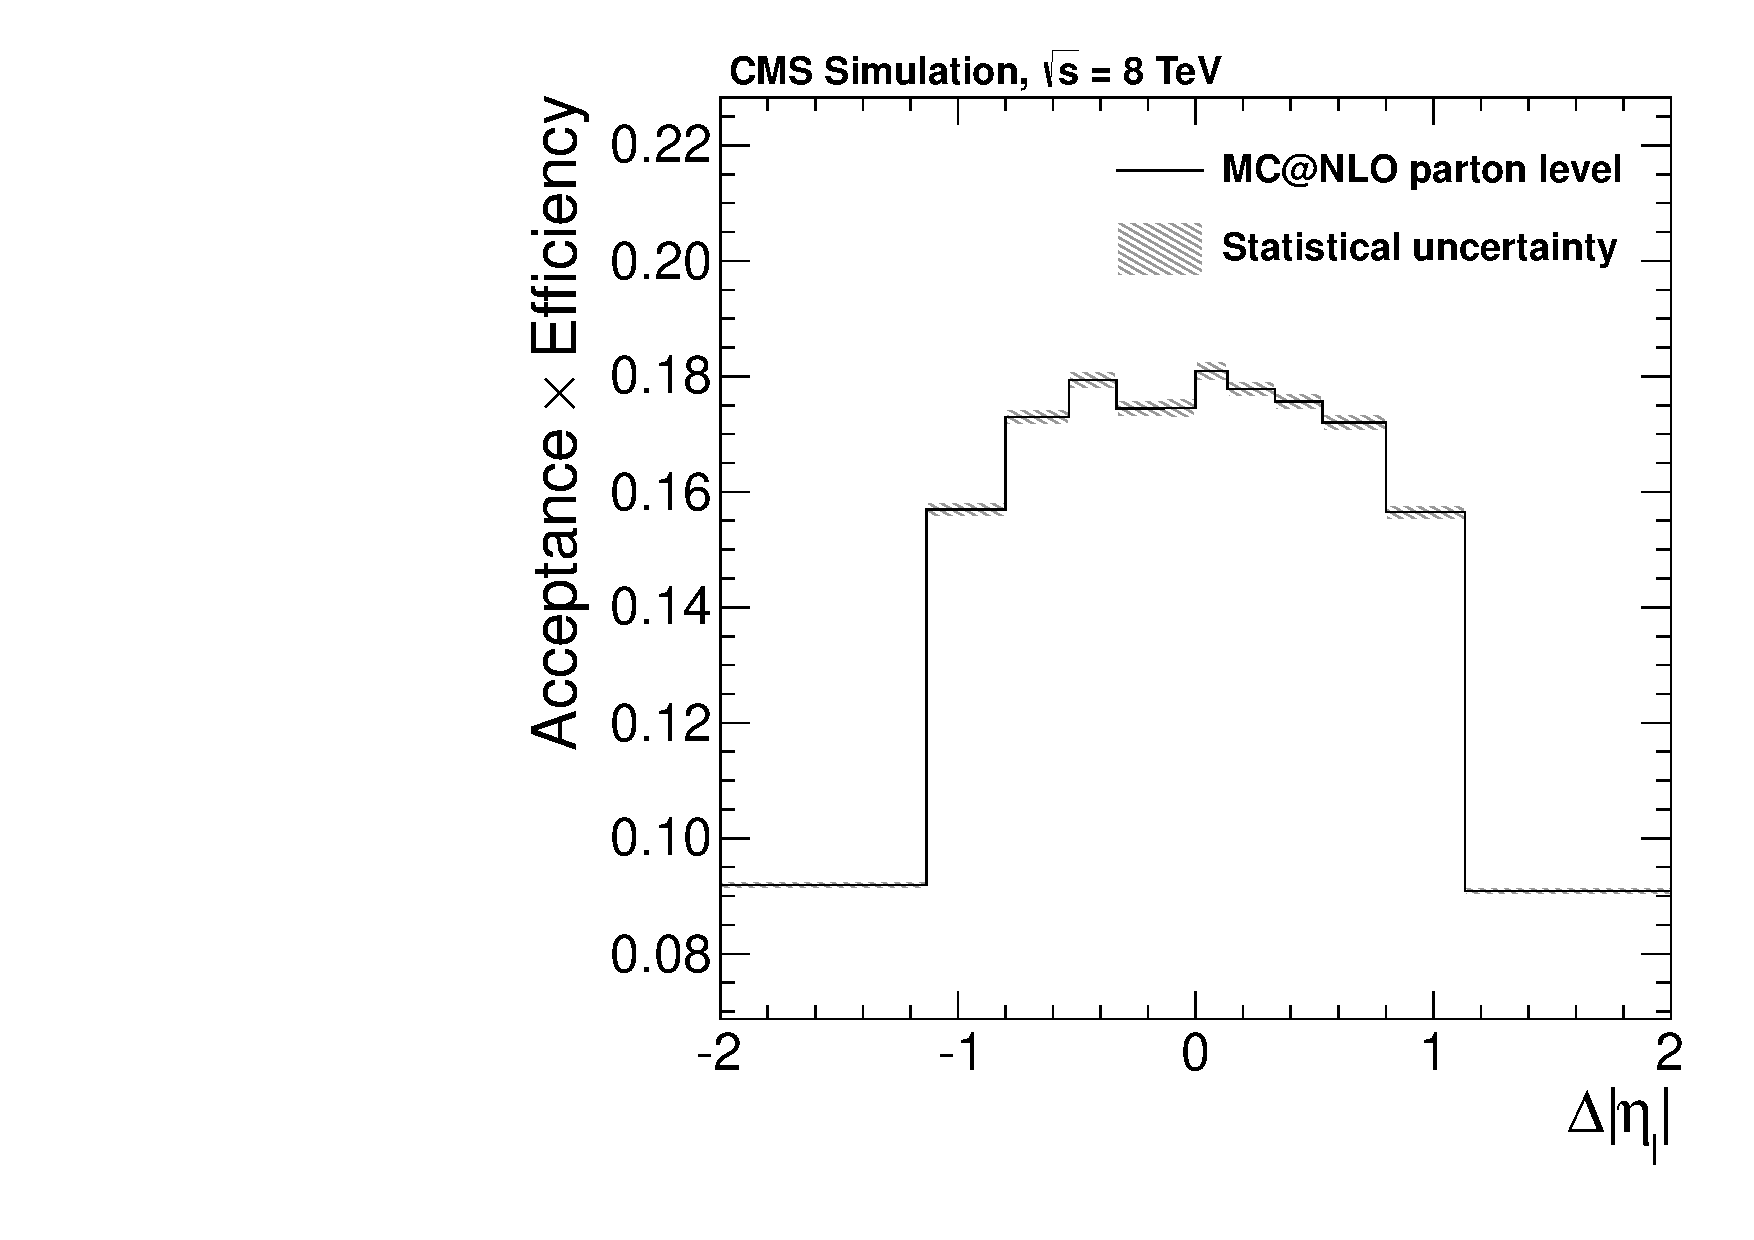
\includegraphics[width=0.325\linewidth]{figures/accept_lepChargeAsym_all.pdf}
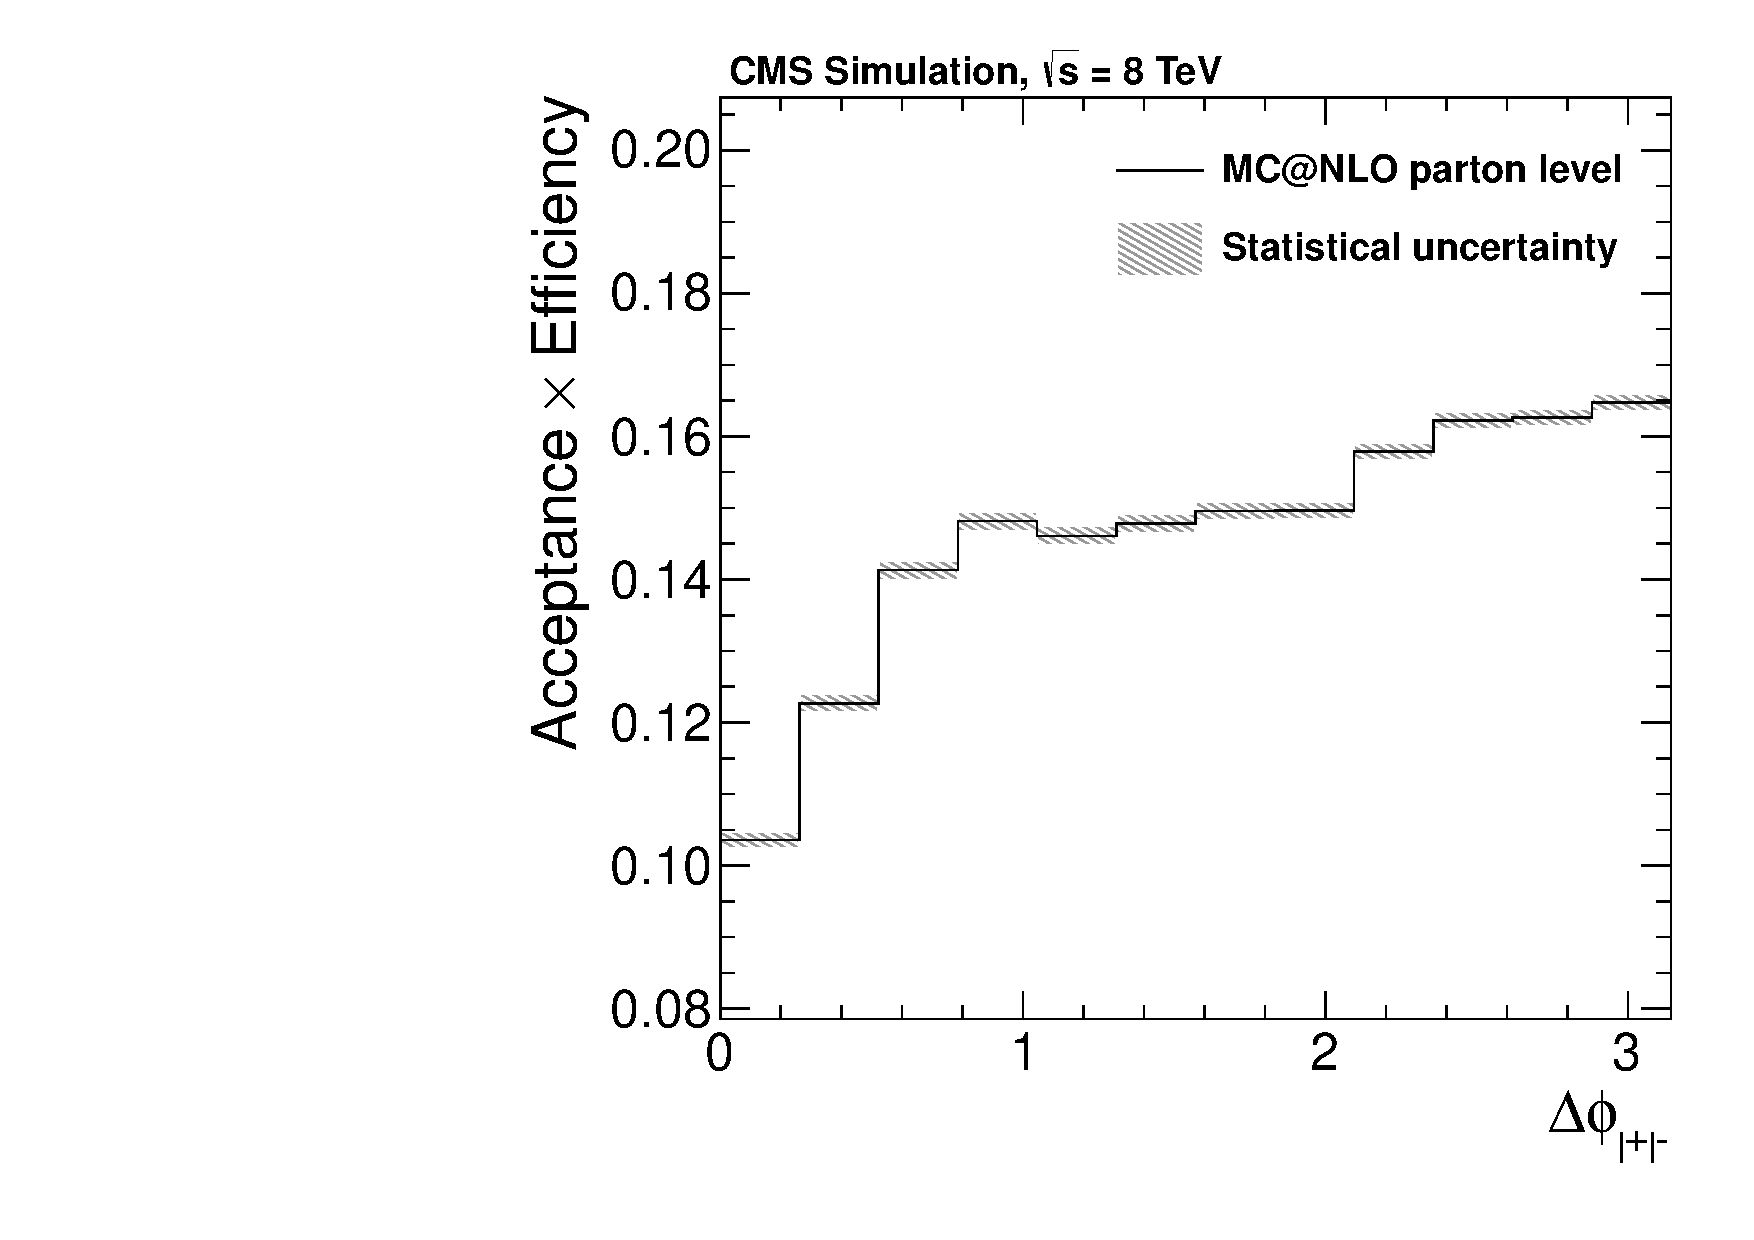
\includegraphics[width=0.325\linewidth]{figures/accept_lepAzimAsym2_all.pdf}
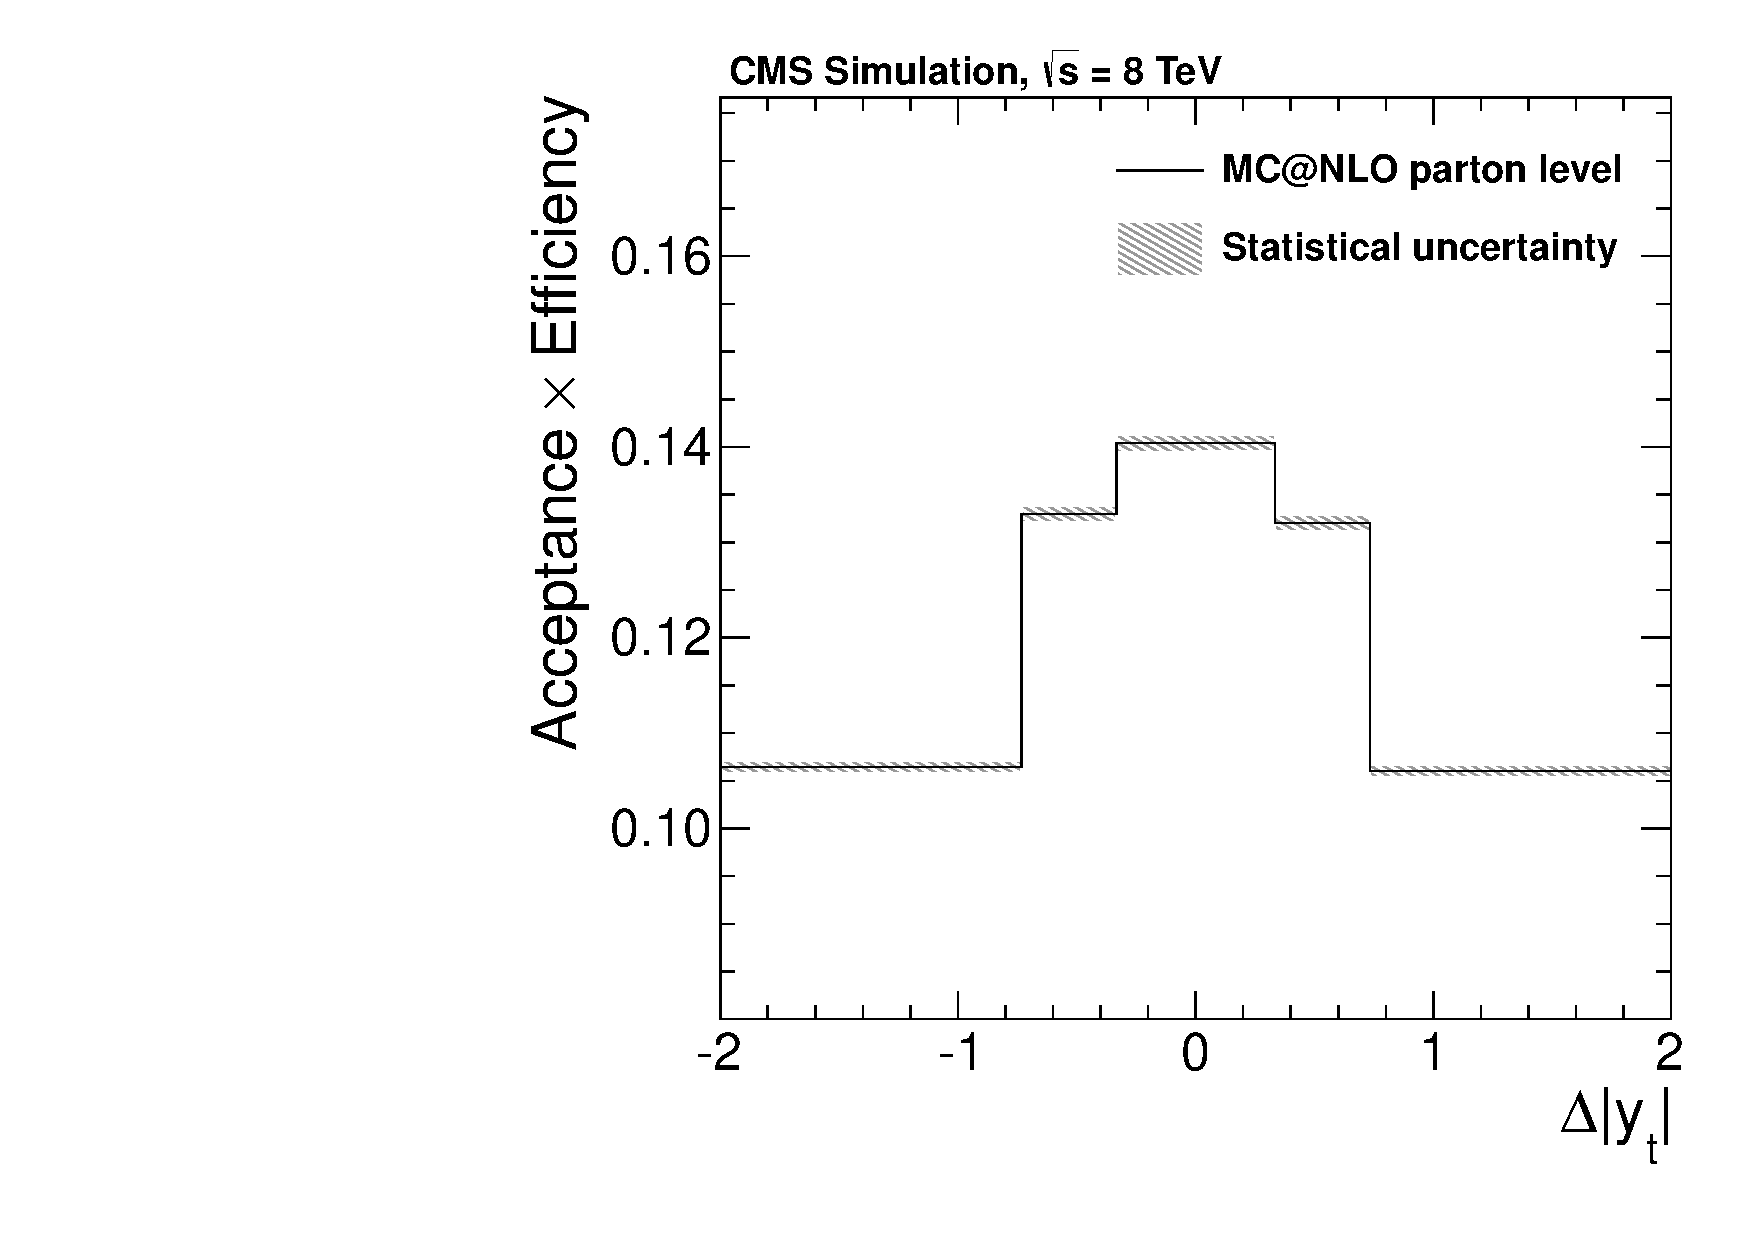
\includegraphics[width=0.325\linewidth]{figures/accept_rapiditydiffMarco_all.pdf}
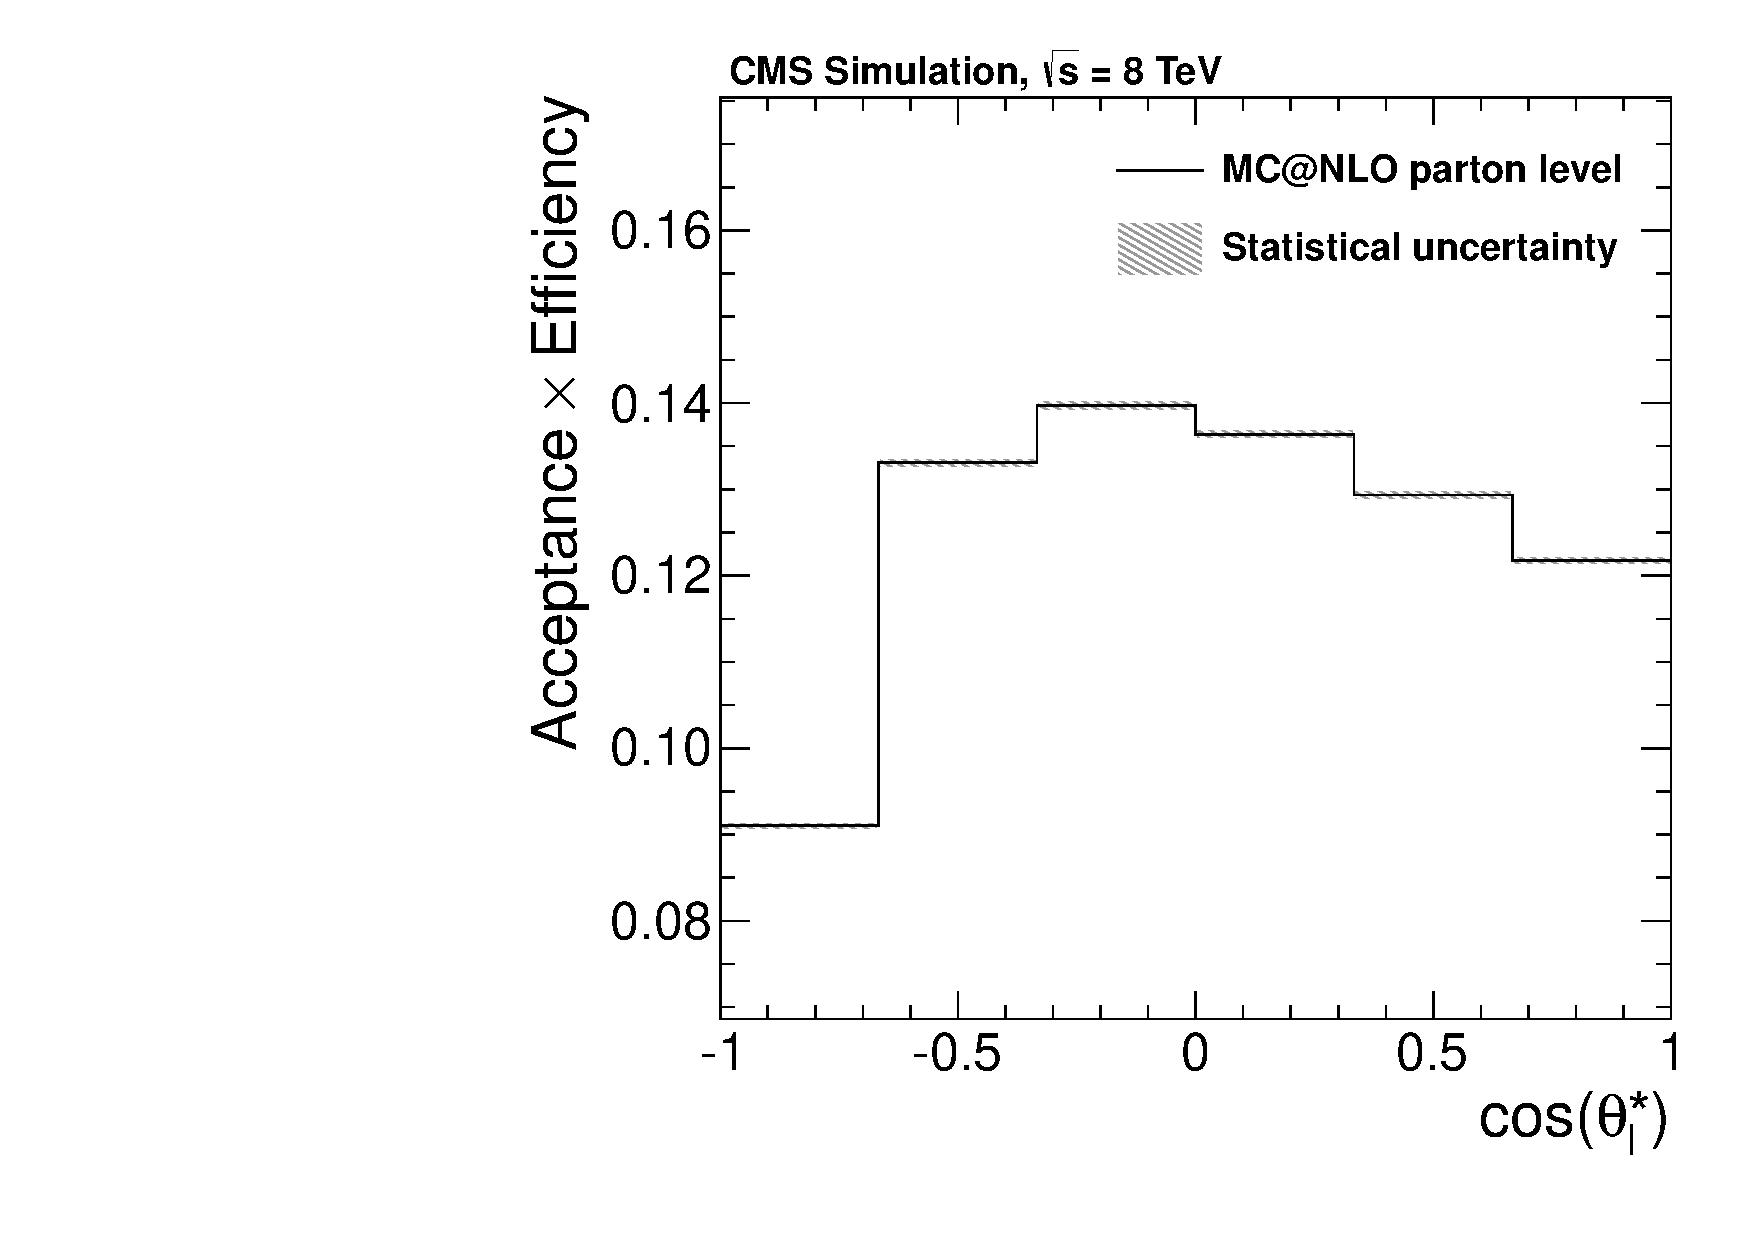
\includegraphics[width=0.325\linewidth]{figures/accept_lepCosTheta_all.pdf}
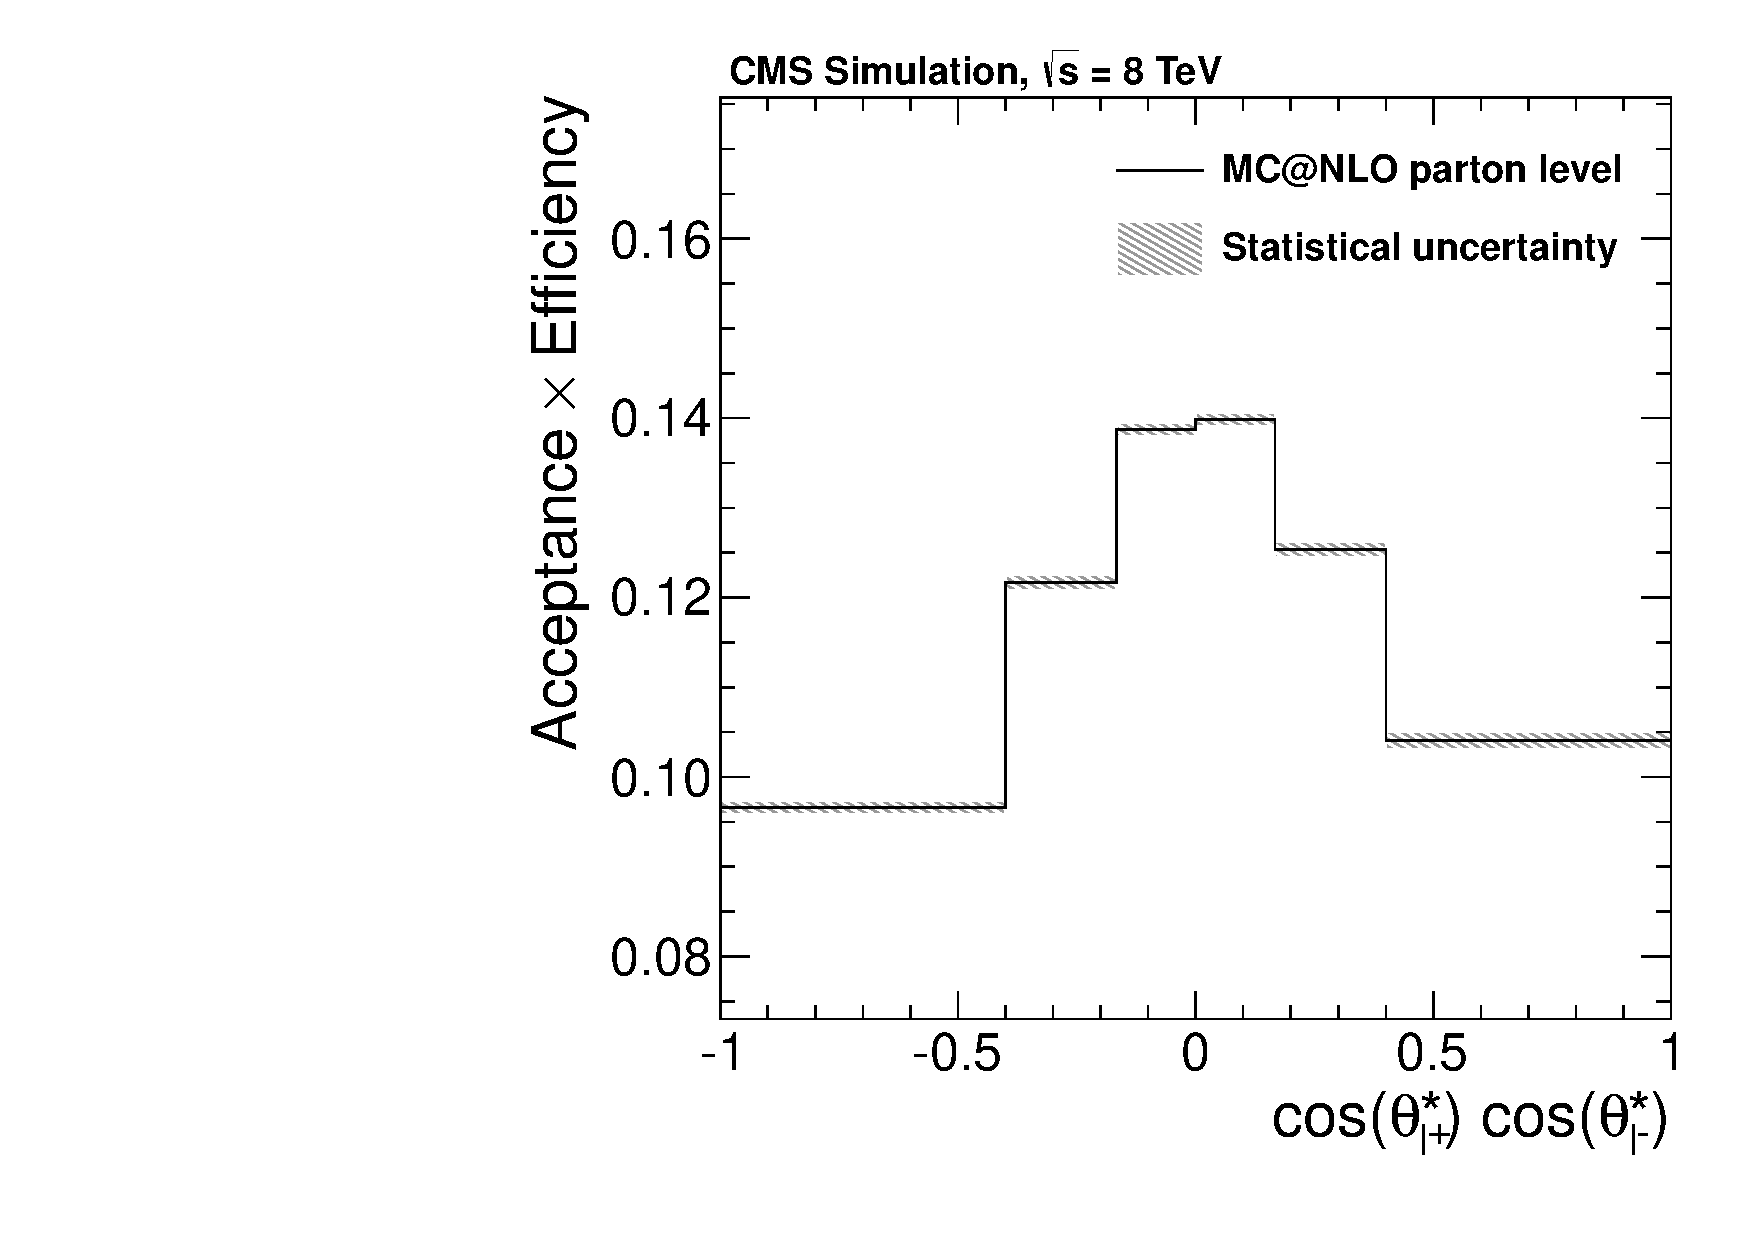
\includegraphics[width=0.325\linewidth]{figures/accept_topSpinCorr_all.pdf}
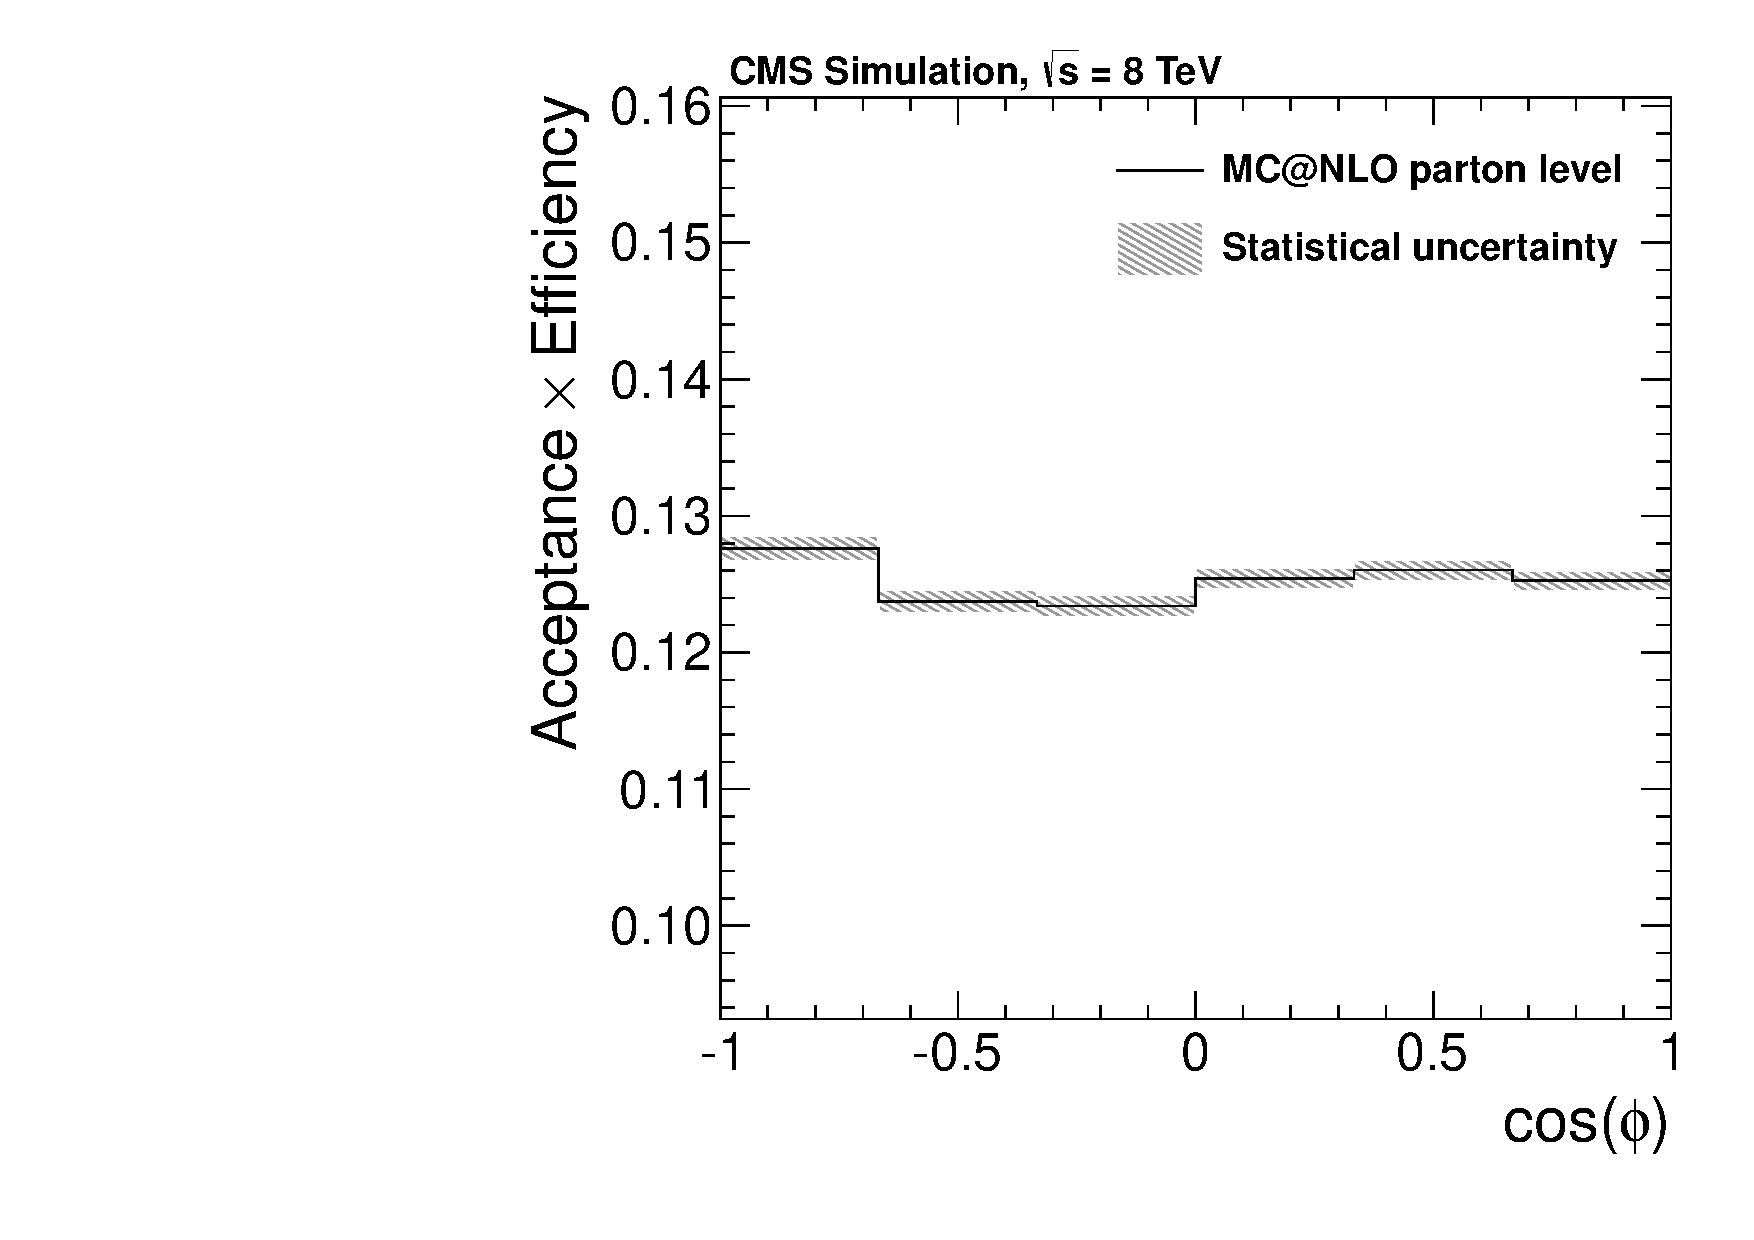
\includegraphics[width=0.325\linewidth]{figures/accept_lepCosOpeningAngle_all.pdf}
\caption{Acceptance matrices for the six asymmetry variables. Since
  all off-diagonal elements are zero, only the diagonal elements are shown.}
\label{fig:afb:acceptance}
\end{center}
\end{figure}

The smearing matrices $S$ were populated as one might expect. Each event
was placed into a 2D histogram bin based on its gen-level asymmetry
(y-axis) and its reco-level asymmetry (x-axis). So each bin in the
histogram corresponds exactly to a single element in the smearing
matrix. These histograms are presented in Figure \ref{fig:afb:smearing}. The smearing
matrices for the leptonic variables have almost no off-diagonal
components, reflecting the high quality of our lepton
reconstruction. For the variables that require $\ttbar$ system
reconstruction, the smearing is noticeable, and may be due to detector
effects or to the limitations of the $\ttbar$ reconstruction
software. At any rate, these smearing matrices are nearly symmetric
about the diagonal. This fact indicates that reconstruction introduces
little to no bias, and simply dilutes the true asymmetry.

% Smearing matrices taken from AN-14-146. Not published in papers.
\begin{figure}[htpb]
\begin{center}
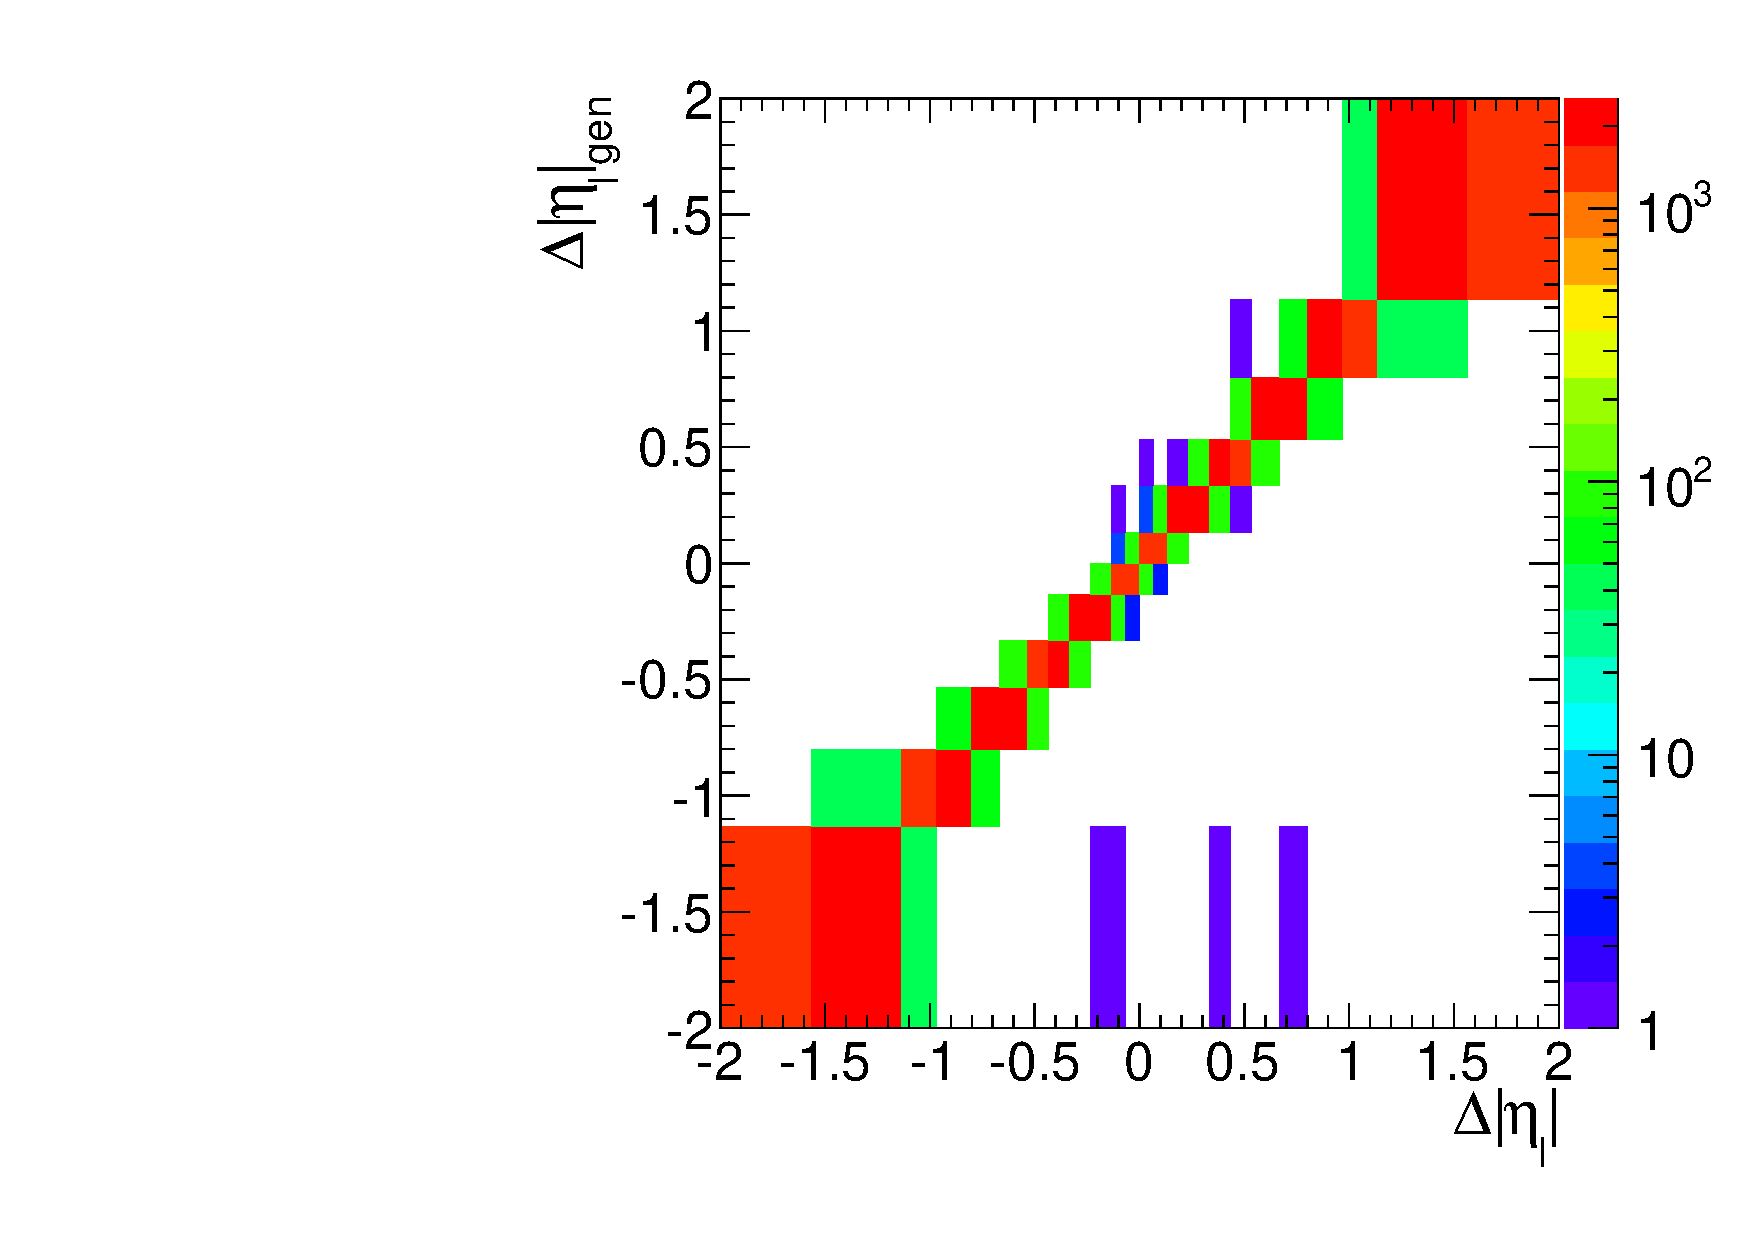
\includegraphics[width=0.325\linewidth]{figures/smearing_lepChargeAsym_all.pdf}
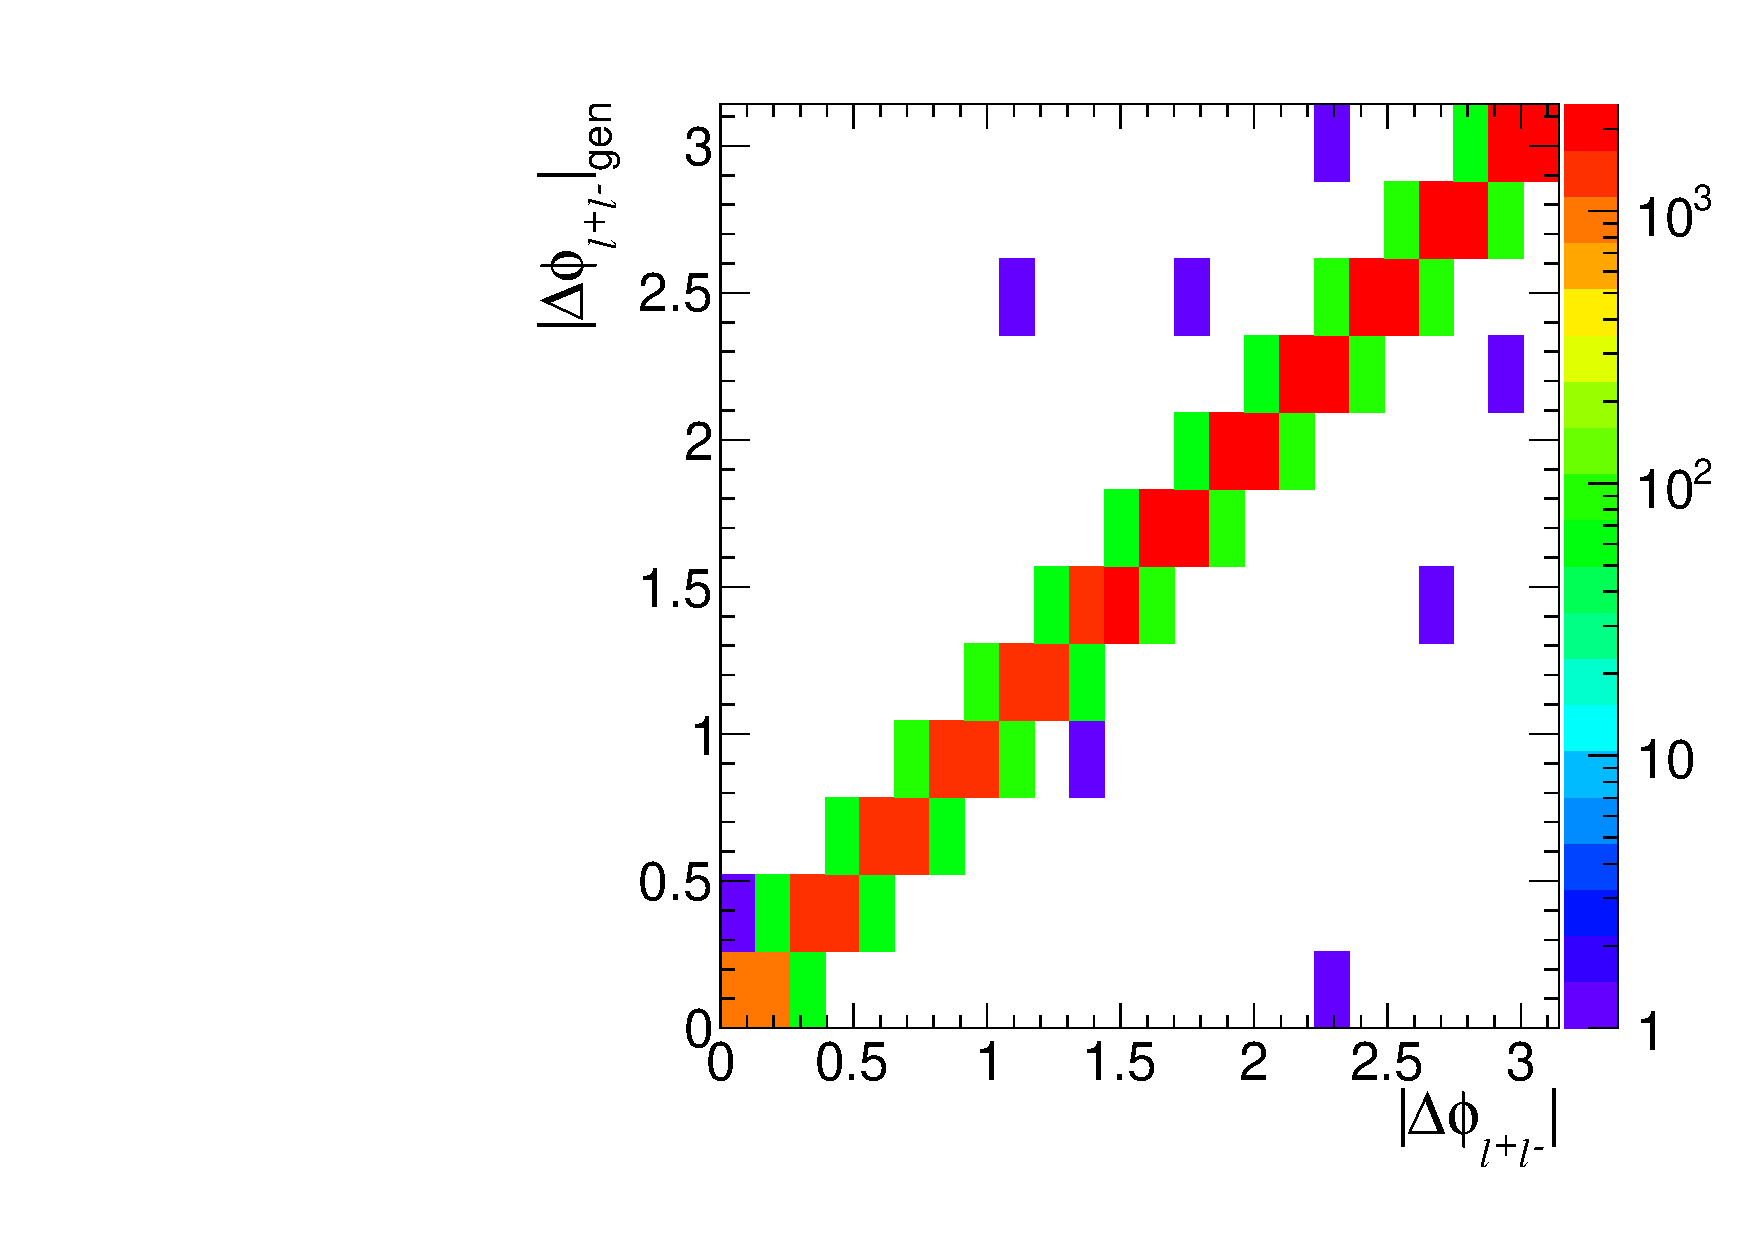
\includegraphics[width=0.325\linewidth]{figures/smearing_lepAzimAsym2_all.pdf}
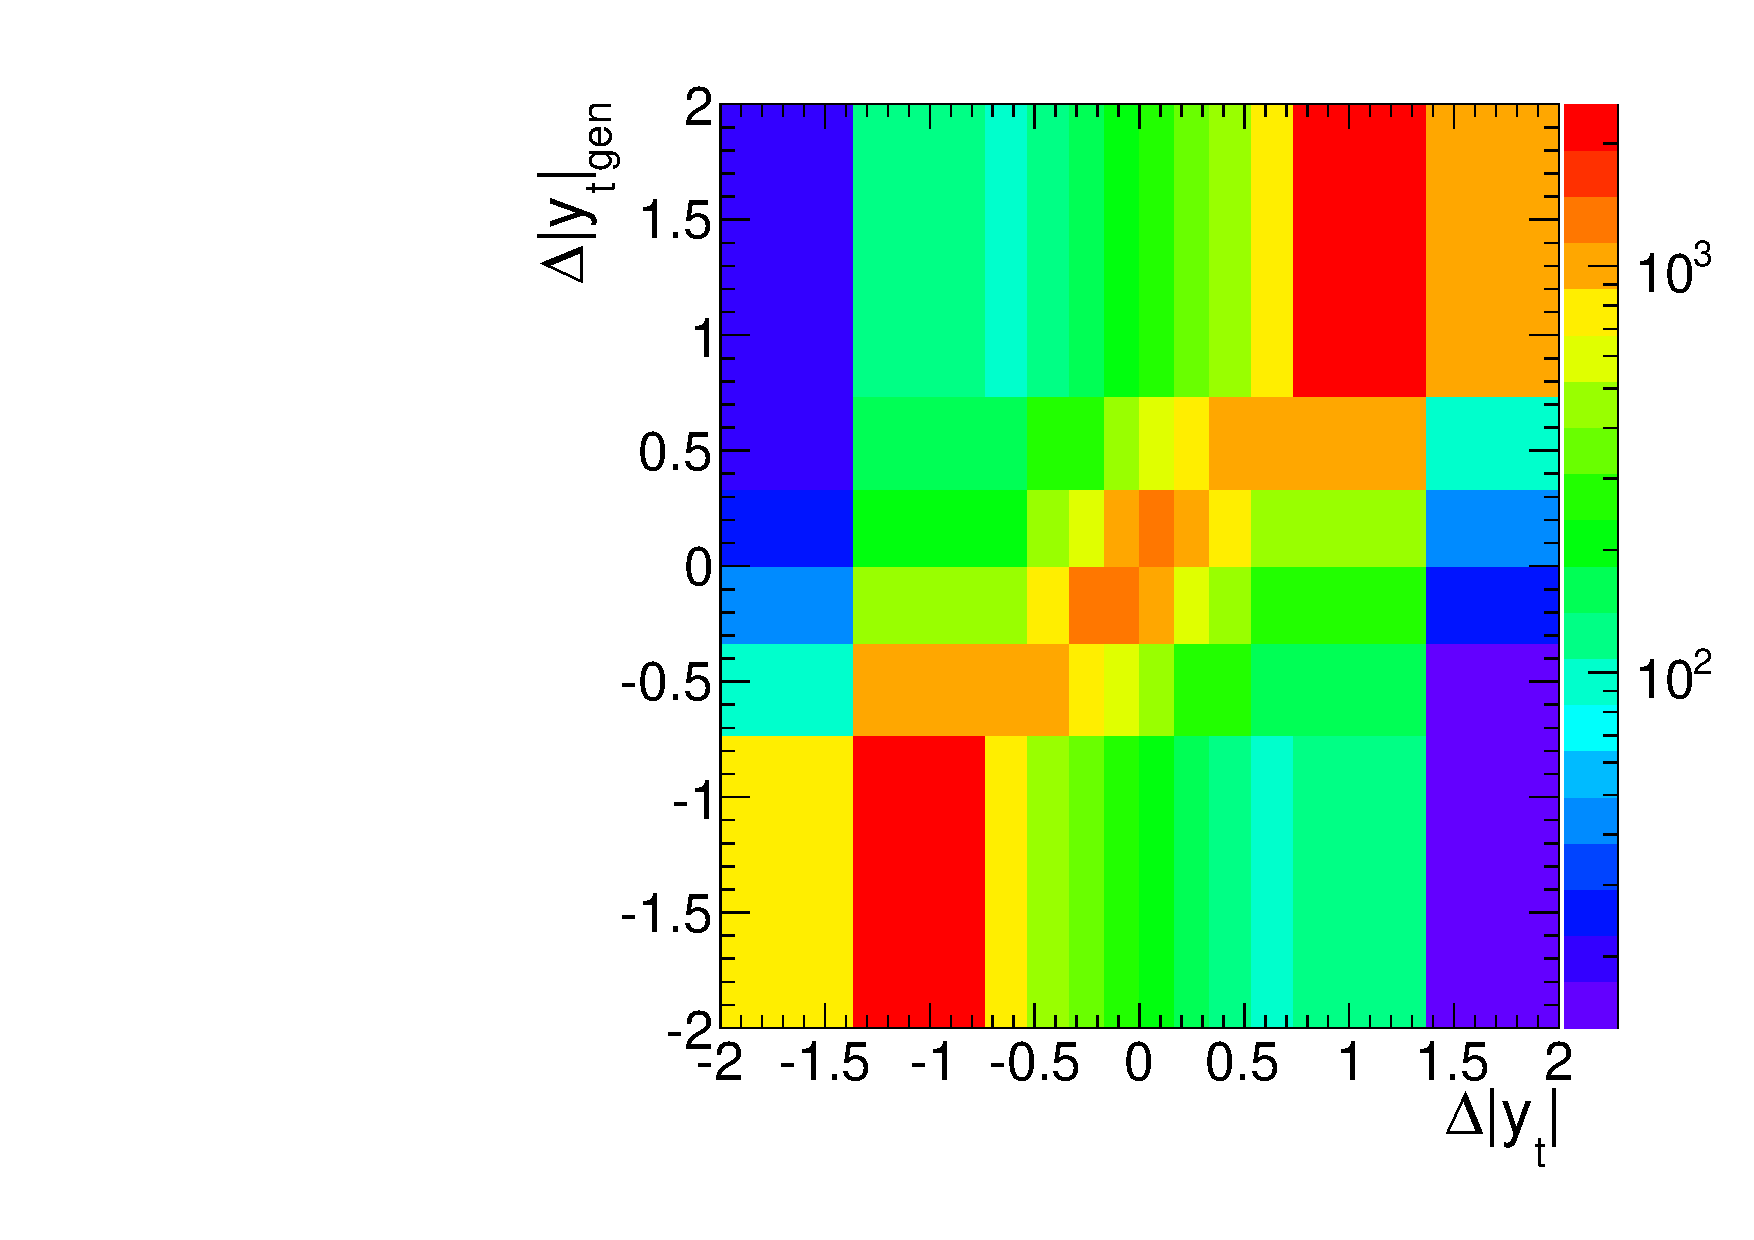
\includegraphics[width=0.325\linewidth]{figures/smearing_rapiditydiffMarco_all.pdf}
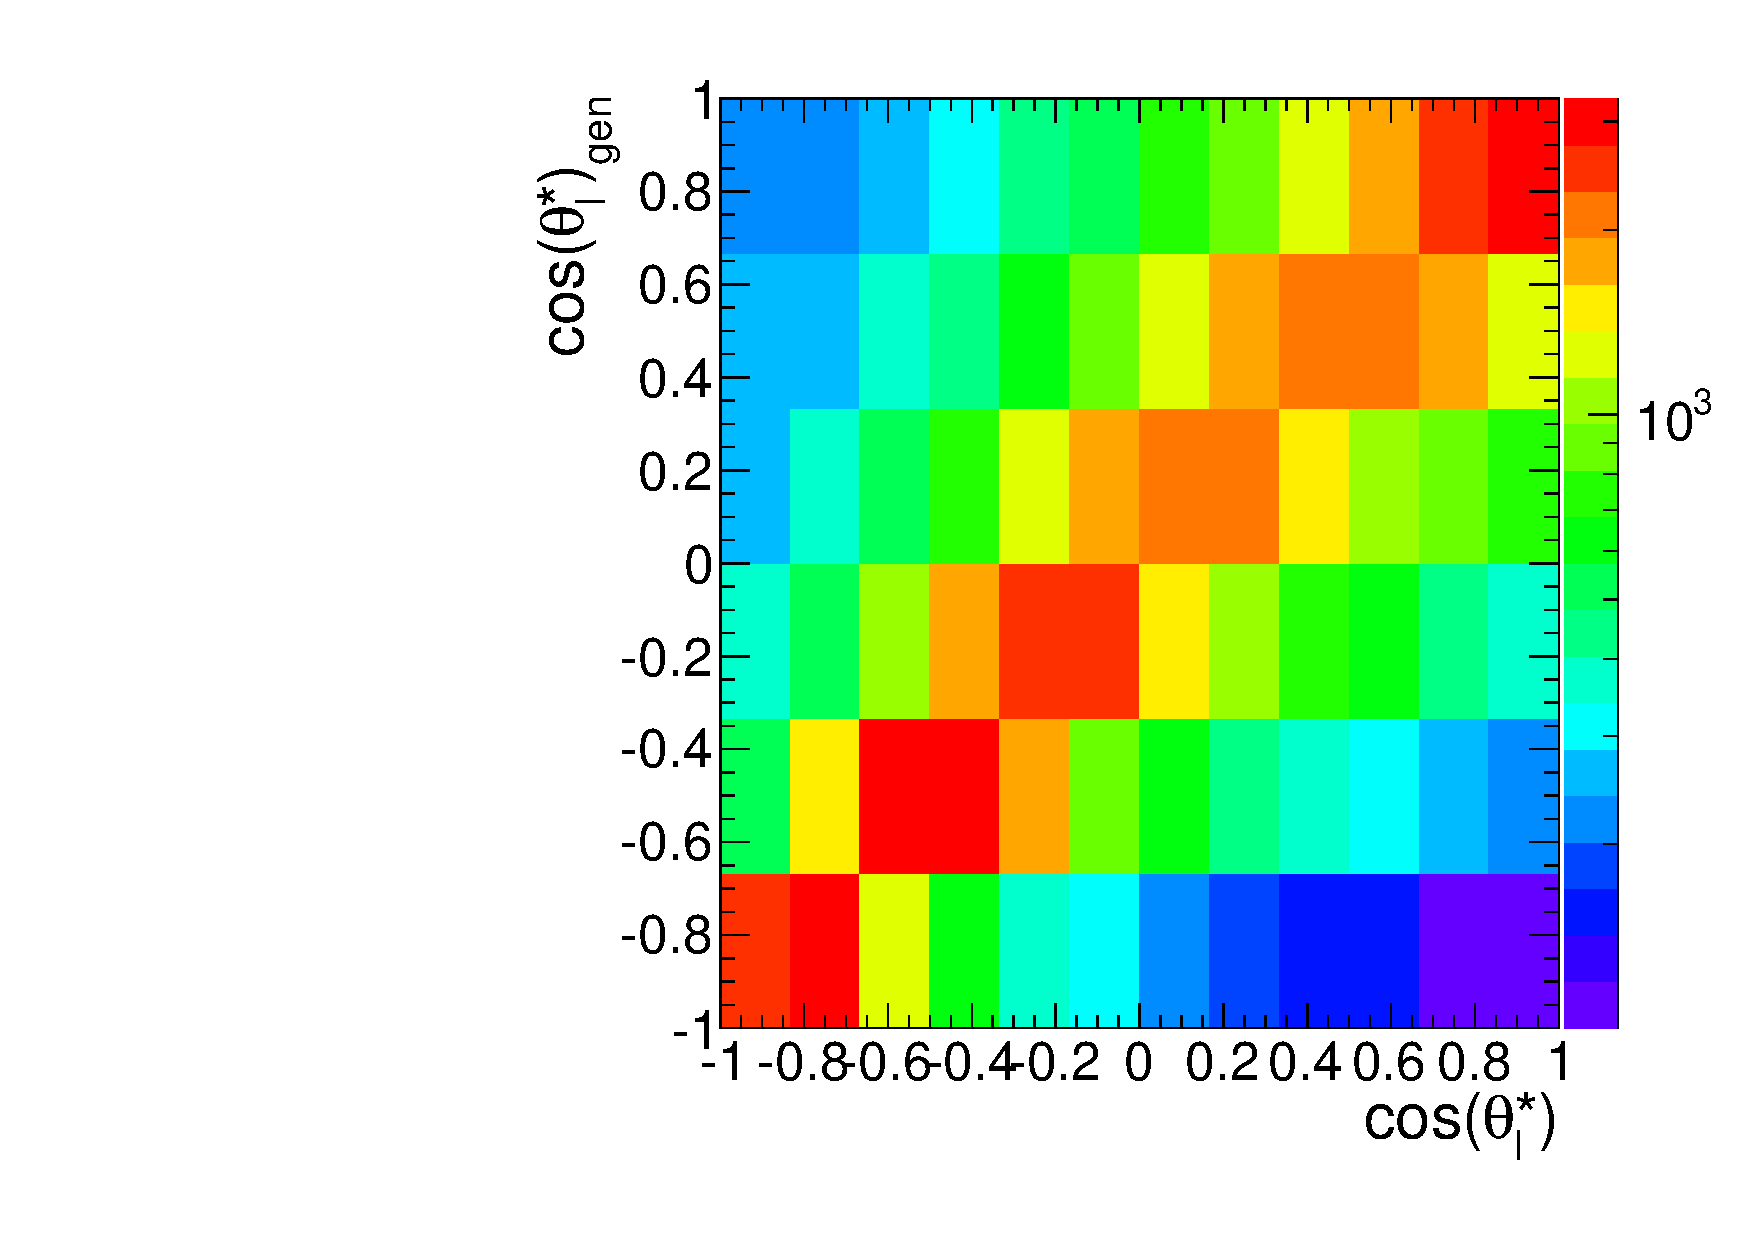
\includegraphics[width=0.325\linewidth]{figures/smearing_lepCosTheta_all.pdf}
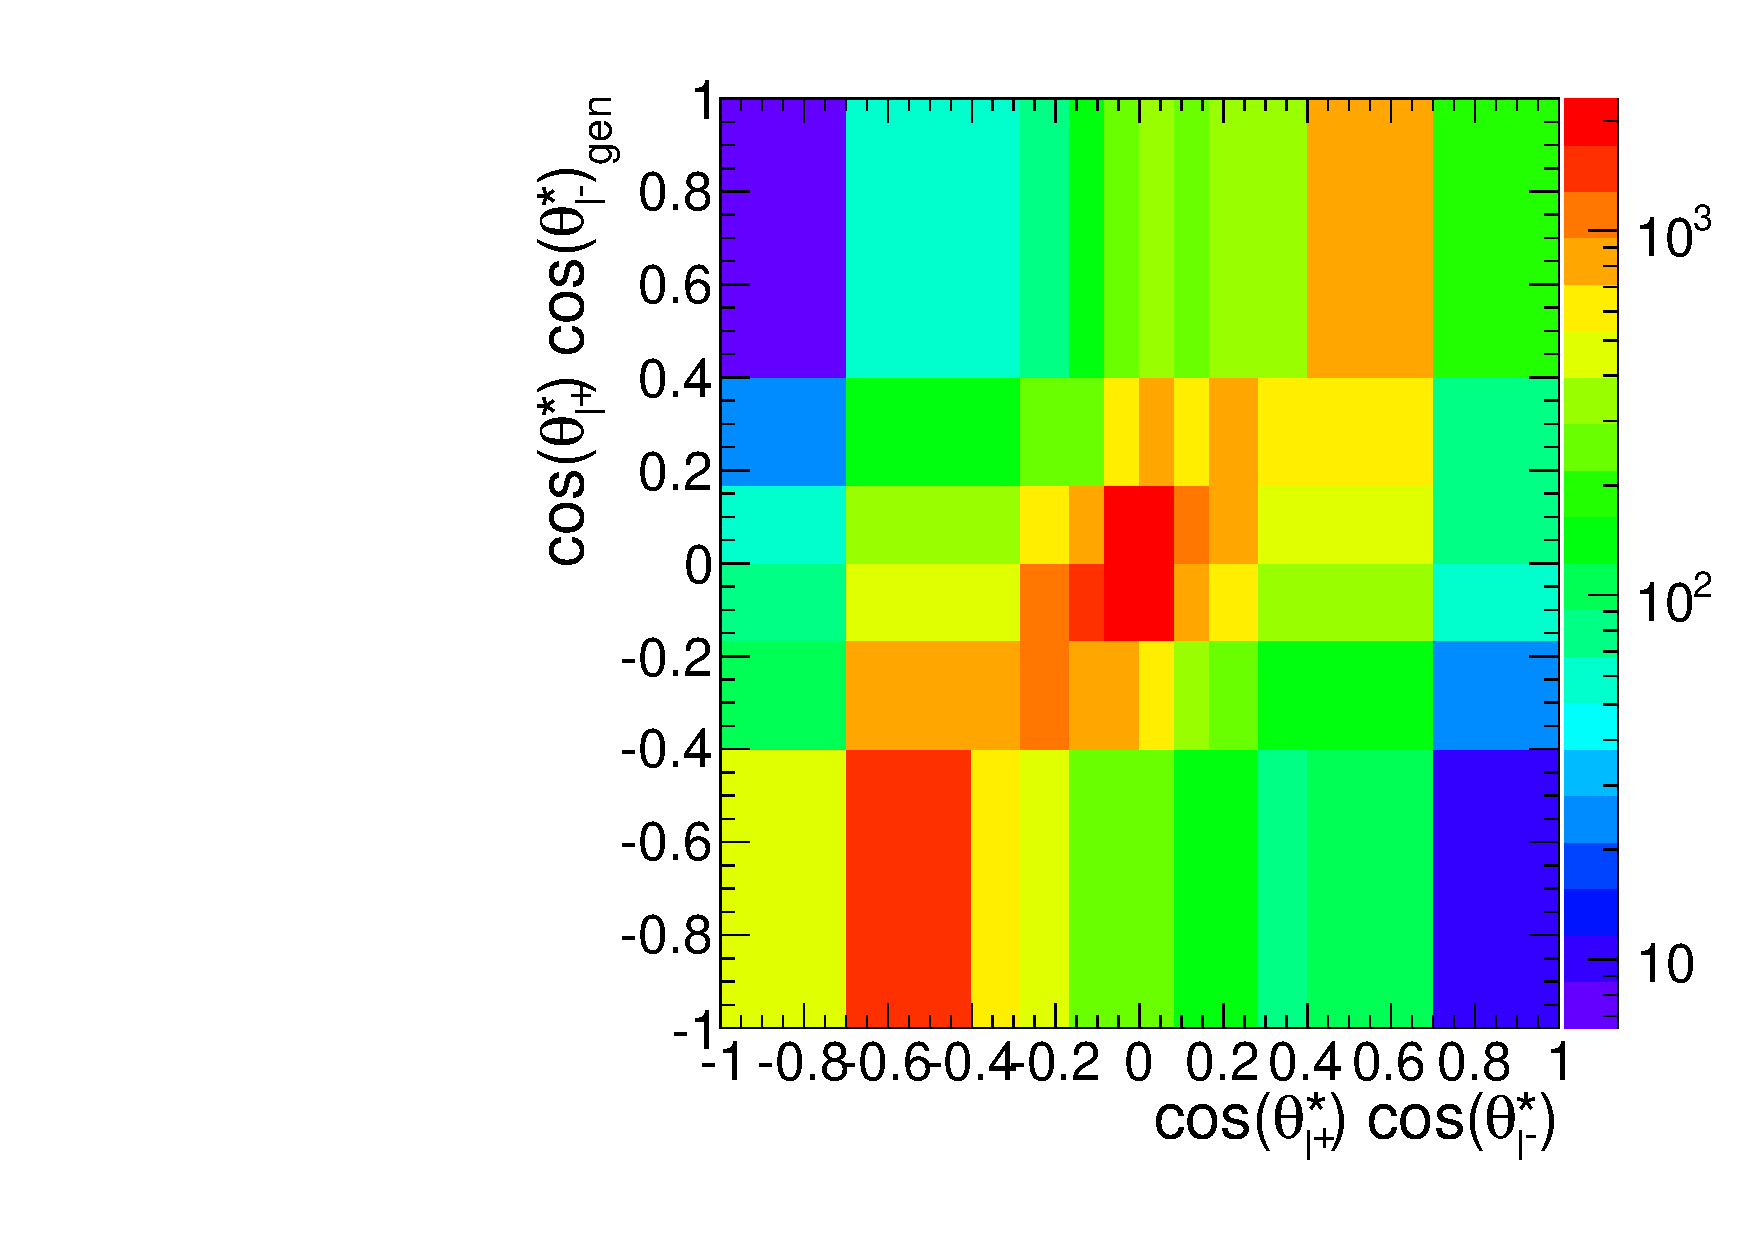
\includegraphics[width=0.325\linewidth]{figures/smearing_topSpinCorr_all.pdf}
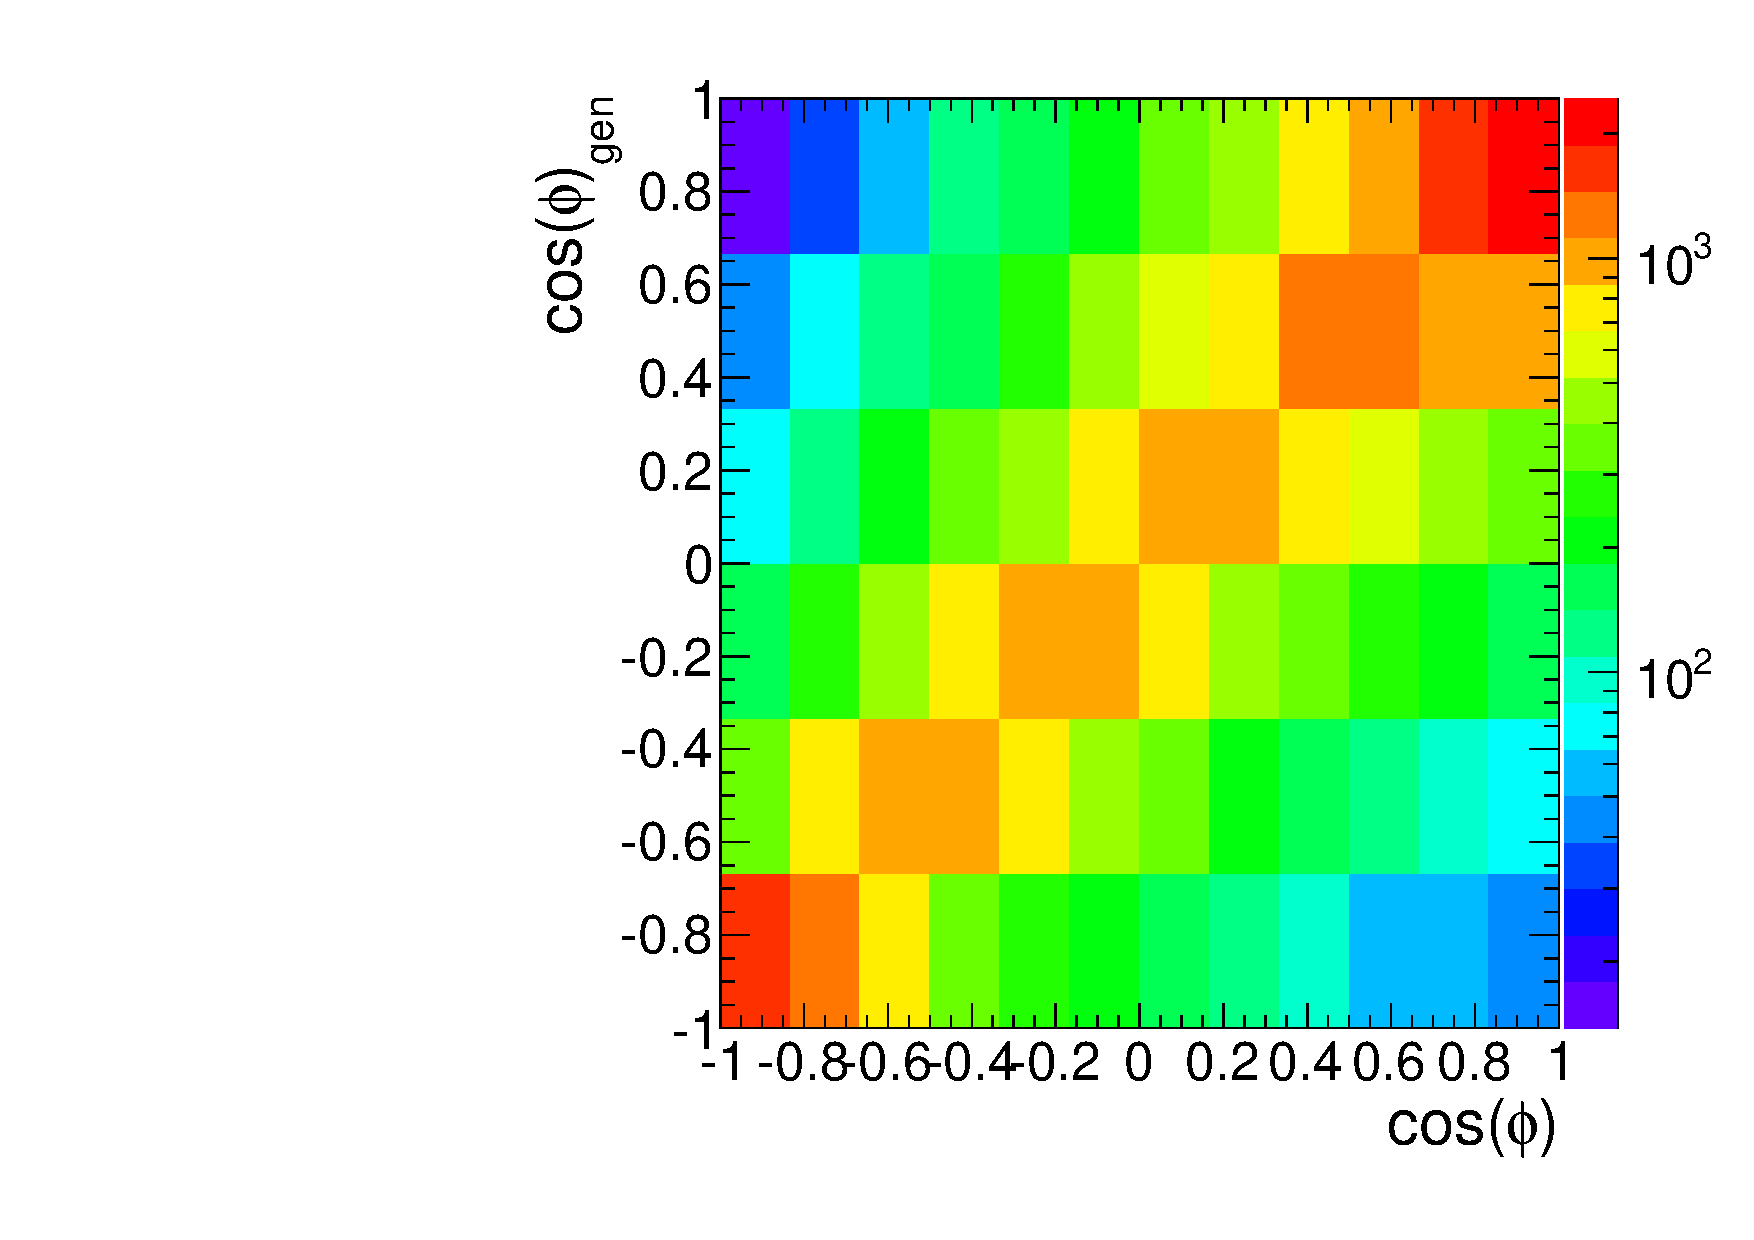
\includegraphics[width=0.325\linewidth]{figures/smearing_lepCosOpeningAngle_all.pdf}
\caption{Smearing matrices for the six asymmetry variables.}
\label{fig:afb:smearing}
\end{center}
\end{figure}

As described in Section \ref{ssec:afbunfoldingbkg}, the choice of the
parameter $\tau$ will impact both the amount of statistical
fluctuation in the unfolded distribution, and the amount of
bias. There are many ways to choose the optimal value of this parameter. We
use the method of minimizing the mean of the global correlation
coefficients, which is also favored by Blobel
\cite{blobelseminar}. The values of $\tau$ we arrived at in this way
are presented in Table \ref{tab:afb:tau1d}. To validate these values,
we checked how the asymmetry and its uncertainties varied as we raised
and lowered tau by up to a factor of 100. As expected, the
uncertainties became larger as $\tau$ was lowered, and the asymmetry % Do I need to include these plots?
central value shifted, indicating bias, as tau was raised. From this, we deduce
that our choices for $\tau$ were appropriate.

% Table of tau values from AN-14-246. Believed unpublished. %%%%%%%%%%%%%%%%%%%%%%%%%%%%
\begin{table}[htb]
\begin{center}
\caption{Optimal $\tau$ values chosen for each asymmetry.}
\label{tab:afb:tau1d}
\begin{tabular}{l | c  c  c  c  c  c }
\hline
Asymmetry & $A_{lepC}$ & $A_{\Delta\phi}$ & $A_{C}$ & $A_{P}$ & $A_{c1c2}$ & $A_{\cos\phi}$ \\ \hline
$\tau$ value & 0.000185 & 0.000166 & 0.000110 & 0.000075 & 0.000089 & 0.000098 \\ \hline
\end{tabular}
\end{center}
\end{table}

\subsection{Two-Dimensional Unfolding Procedure}
\label{ssec:afbunfolding2d}

Describe how we used 2D unfolding to measure differential asymmetries.
Talk about binning choices and other optimizations.
Creating S and A matrices (if any different from 1D)
Choosing the tau parameter

% Binning table from AN-14-246. Believed unpublished, but these values could probably be deduced from published plots.
% \begin{table}[htb]
% \begin{center}
% \caption{Bins chosen for kinematic variables in 2D unfolding.}
% \label{tab:afb:binning2d}
% \begin{tabular}{l |  c  c  c }
% \hline
% Secondary Variable &  B1  &  B2 &  B3 \\ \hline
% $m_{t \bar t}$ (GeV)    &  [0, 430]  &  [430,530]  &  [530,$\infty$]  \\ \hline
% $p_{T}^{t \bar t}$ (GeV)    &  [0,41]  &  [41,92]  &  [92,$\infty$] \\ \hline
% $|y_{t \bar t}|$        &  [0,0.34]  &  [0.34,0.75]  &  [0.75,$\infty$] \\ \hline
%  \hline
% \end{tabular}
% \end{center}
% \end{table}

\subsection{Validation}
\label{ssec:afbunfoldingtests}

Address the concern of introducing bias.
Talk about the linearity and pull tests, and how they quantify any bias
introduced by regularization.
Give the values from those tests.

\section{Systematic Uncertainties}
\label{sec:afbsystematics}

Describe all the systematic uncertainties we calculated.

\section{Results and Interpretation}
\label{sec:afbresults}

\subsection{One-Dimensional Results}
\label{ssec:afbresults1d}

Give the 1D results

\subsection{Two-Dimensional Results}
\label{ssec:afbresults2d}

Give the 2D results

\subsection{BSM Interpretation}
\label{ssec:afbresultsbsm}

Not sure if this section should be included or not. If I keep it:
Talk about the search for chromo-magnetic dipole moments.

\subsection{Acknowledgements}
Mention work of CMS collaboration, maybe specific people who worked on
the analysis with me, and definitely Bernreuther and Si
